\section*{Guide to the appendices}
Appendix~\ref{app:deviations} records the analysis plan, its amendments and the deviations log.
Appendix~\ref{app:ltt} defines the guaranteed threshold rules and proves the proposition of Section~\ref{sec:rules}.
Appendix~\ref{app:results} collects the supporting results, grouped by the question they support; each group opens with
what was done, why, and what it shows. RQ1 and EQ4 are reported in full in the main text. Appendix~\ref{app:prompts} shows
the requests sent to the models, and Appendix~\ref{app:memorization} describes the memorization probe.

\section{Analysis plan, amendments and deviations}
\label{app:deviations}

The analysis plan (v1.0) fixed the tasks, splits, decision units, metrics, primary rule and contrasts before any test-split
outcome was computed. Four amendments were each recorded before the data they govern. The plan was kept in the project
repository rather than registered externally:
\begin{itemize}
  \item \textbf{v1.1} added OpenAI Decisions as a confirmatory coder, Qwen3.5-9B as a non-reasoning token-probability
  comparator, and the A3 analyses (recalibration, per-code thresholds, risk control, cascades).
  \item \textbf{v1.2} added Clef, Clef-flash, pplx-decider, Kev-9B and Kev-27B as a confirmatory family, with the
  same-base contrasts pre-specified as secondary.
  \item \textbf{v1.3} added the memorization probe.
  \item \textbf{v1.4} added the prompt-sensitivity check.
\end{itemize}
The deviations log records eighteen entries; everything added or changed after results were seen is exploratory. In summary:
\begin{enumerate}
  \item A response-cache key ignored option order. It was fixed and the affected order arms were re-run before analysis.
  \item Adjudication moved from a single human pass to a blinded two-family LLM panel plus the author on disputed items.
  \item The author completed 48 of 72 assigned adjudications.
  \item The RQ5 code-type labels were assigned by the assistant from definition text, after some per-code results had been seen.
  \item OpenAI Decisions collection notes, including its exact invariance to question order on multi-label tasks.
  \item The Qwen model was chosen by availability without third-party data sharing; Qwen3.8-2.4T was added on a subset; a
  null-logprob parse fix was made before any full-run data.
  \item The A3 implementation details were fixed after the primary results had been seen.
  \item A3 was revised after its first output: a power-based LTT start, oracle thresholds and a restructured per-code
  head-to-head. All A3 results are therefore exploratory.
  \item Sonnet was extended from a nested subset to the full sample after the subset results had been seen.
  \item The repeatability check, Sonnet's robustness arms and the Holm sensitivity analysis were added.
  \item Kev-27B was limited to the main and format arms.
  \item Kev-9B's robustness arms cover one to four tasks per arm: the hosting workspace was disabled partway through.
  \item The decision-model committee and new cascades were added, exploratory, and fixed before computation.
  \item A decoy-name control was added for flagged memorization cells.
  \item The author later reviewed those labels and approved them unchanged, after the RQ5 results had been computed.
  \item After an external review of the first draft: a cluster-level guarantee replaced LTT on decisions, with joint
  certification for cascades and split samples for learned scores; the prevalence analysis, the category-only control,
  adjudication by verdict source, the feasibility calculation and a text-free spend ledger were added; RQ3 point estimates
  were design-weighted; three reporting errors were fixed.
  \item After a second review: the guarantee was recast for a fixed corpus (corpus LTT), with the earlier test kept as LTT
  on i.i.d.\ clusters; related tasks share bootstrap draws; the Sonnet subset contrast is the confirmatory one; the probability
  floor moved to $10^{-12}$, and Platt maps became the recalibration yardstick.
  \item After a third review: the betting tests average over random visiting orders; the budget curves, bootstrap streams and
  prompt-sensitivity intervals were corrected; the feasibility bound and the single-utterance design were added; prose
  intervals are generated from the results files.
\end{enumerate}
The full log, plan and amendments are in the released repository.

\section{Guaranteed threshold rules}
\label{app:ltt}

\paragraph{LTT on decisions.} Thresholds are tested from the most confident tie block downwards with binomial tests of
``risk $>\varepsilon$'' at level $\delta=0.05$, stopping at the first failure; the sequence starts at the first block with at least
124 decisions. Errors are scaled to Kish's effective sample size \citep{kish1965survey}, which gives fractional counts. The test
treats decisions as independent and fails when they are not (Table~\ref{tab:tab20_ltt_simulation}).

\paragraph{Corpus LTT.} A corpus has $N$ clusters; $n$ of them, chosen uniformly at random, are hand-coded. Fix the scores, the
grid $\{0.5, 0.55, \dots, 0.9, 0.925, 0.95, 0.97, 0.98, 0.99, 0.995, 1.0\}$ and $B$, the largest total weight of one cluster in
the corpus. For threshold $t$, every cluster has a fixed value $Y_i=(Z_i+\varepsilon B)/B\in[0,1]$ with
$Z_i=\sum_j w_{ij}\mathbf{1}\{c_{ij}\ge t\}(e_{ij}-\varepsilon)$; let $\mu$ be their corpus mean and $\bar Y$ the mean over the
hand-coded clusters. The uncoded remainder has error at most $\varepsilon$ among its accepted decisions exactly when its
$Z$-sum is at most 0, that is, when $\mu\le m^\ast=((N-n)\varepsilon+n\bar Y)/N$.

To test ``$\mu\ge m$'', visit the hand-coded clusters in a uniformly random order, drawn independently of the labels; the
clusters visited are then a uniformly random sample drawn without replacement, in draw order. Under that null, the $k$th
cluster's value has conditional mean $(N\mu-S_{k-1})/(N-k+1)\ge \mu_k(m)=(Nm-S_{k-1})/(N-k+1)$, where $S_{k-1}$ is the sum of
the values already seen. So $K_k=\prod_{i\le k}\bigl(1-\nu_i\,(Y_i-\operatorname{clip}(\mu_i(m),0,1))\bigr)$, with predictable
bets $\nu_i=\min\{1,\sqrt{2\log(1/\delta')/(n\hat\sigma^2_{i-1})}\}\in[0,1]$, is a non-negative supermartingale
\citep{waudbysmith2024betting}. The variance estimate is the plug-in rule with a pseudo-observation: $\hat\sigma^2_0=1/4$ and,
for $i\ge1$, $\hat\mu_i=(1/2+\sum_{j\le i}Y_j)/(i+1)$ and $\hat\sigma^2_i=(1/4+\sum_{j\le i}(Y_j-\hat\mu_j)^2)/(i+1)$. The bets
use only values already seen and do not depend on $m$; validity needs only that, but power, and hence the feasibility numbers
below, depends on this choice. Its final value $K_n$ has expectation at most 1: it is an e-value. The order must be
random: a random set visited in a fixed order does not have these conditional means. Rather than rely on one random order, we
draw $R=100$ independent orders and average their final values, $\bar K(m)=R^{-1}\sum_r K_n^{(r)}$.
An average of e-values is an e-value \citep{vovk2021evalues}, so $p(m)=\min(1,1/\bar K(m))$ satisfies $P(p(m)\le\delta')\le\delta'$
under the null by Markov's inequality. Each $K_n^{(r)}$ increases with $m$, so $\bar K$ does too, and rejecting at $m^\ast$
implies rejecting at every larger $m$. If the remainder's error exceeds $\varepsilon$, then $\mu>m^\ast$, so certifying $t$
requires rejecting at $m=\mu$, a true null, which happens with probability at most $\delta'$. Testing each of the 16
thresholds at $\delta'=\delta/16$ gives the proposition in Section~\ref{sec:rules}. The only randomness used is the choice of
clusters to hand-code and the visiting orders; dependence among errors is unrestricted. The orders come from a
pseudo-random generator with a recorded seed, fixed before this analysis and not chosen by any outcome.

\paragraph{LTT on i.i.d. clusters.} For the population target, the same $Y_i$ are tested against the constant null mean
$\varepsilon$ with the same betting process and the same averaging over orders. This is valid if clusters are independent draws whose weights never exceed $B$;
exchangeability alone is not enough, because a shared latent cause can make every cluster right or every cluster wrong
together. For MFRC, $B$ is a genuine bound (eight codes per comment at one weight); for transcripts of unbounded length it is not.

\paragraph{Learned scores and pipelines.} Per-code maps and the prevalence baseline are fitted on half of the calibration
clusters and frozen; corpus LTT runs on the other half, with the corpus taken as that half plus the test split, and the frozen
scores are applied to the test split. A two-stage cascade is one hypothesis per combination of stage thresholds (8 per stage,
plus ``off'' for the second), with Bonferroni over all 72 combinations; the certified combination with the largest calibration
coverage is used.

\paragraph{What the procedure needs.} For a coder that accepts everything and is never wrong, $Y_i=\varepsilon(1-r_i)$ with
$r_i$ the unit's weight relative to $B$, and the conditional null mean at $m^\ast$ is at most $\varepsilon$. Since bets are capped at
1, each unit can multiply the capital by at most $1+\varepsilon r_i$, whatever the order, and certification with the grid needs
the capital to reach $16/0.05=320$. Hence $\sum_{\text{coded}}\log(1+\varepsilon r_i)\ge\log 320$ is necessary for any set of
hand-coded units and any visiting order (Table~\ref{tab:tab21_ltt_feasibility}, ``lower bound''). For MFRC, whose comments
all have the same weight, at least 119 comments are needed; our procedure first certifies after a median of 123. With whole
transcripts as units, where a typical transcript carries 8--27\% of the largest one's weight, the bound rules out
certification on AnnoMI (both tasks) and TalkMoves student even if every transcript but one were hand-coded, and on
TalkMoves teacher it needs at least 388 of 444 lessons. These requirements belong to this procedure (capped bets, scaling by
the largest unit, Bonferroni over the grid) under whole-transcript sampling. Because corpus LTT needs only random selection,
not independence, the unit can be smaller: drawing single utterances or sentences at random, with their context, keeps every
unit's weight close to $B$, and a perfect coder is then certified after a median of 139--163 hand-coded segments
(Table~\ref{tab:tab21_ltt_feasibility}). Table~\ref{tab:tab21b_utterance_sampling} applies that design to the real coders.

\section{Additional results}
\label{app:results}

\subsection{RQ2: uncertainty and human disagreement, in detail}
These tables give the per-coder numbers behind Figure~\ref{fig:rq2} (\S\ref{sec:rq2}): how strongly each coder's uncertainty
tracks the spread of human labels, and how its agreement with annotators compares with each annotator's agreement with the
others. The decision models and the verbalized signals track disagreement; token probabilities and vote shares do not. No
coder falls below the human range, which is broad, so the comparison is descriptive.

\begin{table}[t]
\centering
\small
\caption{RQ2: model uncertainty and human disagreement, by coder (test items with $\geq$ 3 annotators)}
\label{tab:tab05_rq2}
\begin{adjustbox}{max width=\linewidth}
\begin{tabular}{llrrrl}
\toprule
task & signal & \makecell[br]{Spearman: \\{} uncertainty \\{} vs human \\{} split} & \makecell[br]{AUROC: flags \\{} split items} & \makecell[br]{model $\kappa$ \\{} (mean over \\{} references)} & \makecell[bl]{annotators \\{} below model} \\
\midrule
MFRC & Jev & 0.326 & 0.718 & 0.269 & 2 of 6 \\
MFRC & OpenAI Decisions & 0.242 & 0.659 & 0.260 & 2 of 6 \\
MFRC & Luna verbal & 0.339 & 0.721 & 0.250 & 2 of 6 \\
MFRC & Haiku verbal & 0.375 & 0.742 & 0.189 & 1 of 6 \\
MFRC & gpt-oss verbal & 0.307 & 0.673 & 0.310 & 3 of 6 \\
MFRC & Luna logprob & 0.138 & 0.582 & 0.250 & 2 of 6 \\
MFRC & 3-LLM agreement & 0.199 & 0.591 & 0.280 & 2 of 6 \\
MFRC & Sonnet verbal & 0.427 & 0.784 & 0.361 & 5 of 6 \\
MFRC & Clef (27B) & 0.404 & 0.771 & 0.282 & 2 of 6 \\
MFRC & Clef-flash (9B) & 0.395 & 0.764 & 0.306 & 3 of 6 \\
MFRC & pplx-decider & 0.398 & 0.767 & 0.246 & 1 of 6 \\
MFRC & Kev-9B & 0.325 & 0.717 & 0.239 & 2 of 6 \\
MFRC & Kev-27B & 0.394 & 0.764 & 0.249 & 2 of 6 \\
AnnoMI client & Jev & 0.547 & 0.859 & 0.706 & 7 of 10 \\
AnnoMI client & OpenAI Decisions & 0.517 & 0.812 & 0.696 & 7 of 10 \\
AnnoMI client & Luna verbal & 0.514 & 0.803 & 0.701 & 7 of 10 \\
AnnoMI client & Haiku verbal & 0.568 & 0.875 & 0.590 & 3 of 10 \\
AnnoMI client & gpt-oss verbal & 0.522 & 0.817 & 0.655 & 7 of 10 \\
AnnoMI client & Luna logprob & -0.100 & 0.462 & 0.701 & 7 of 10 \\
AnnoMI client & 3-LLM agreement & 0.324 & 0.604 & 0.648 & 7 of 10 \\
AnnoMI client & Sonnet verbal & 0.647 & 0.872 & 0.714 & 9 of 10 \\
AnnoMI client & Clef (27B) & 0.636 & 0.904 & 0.508 & 1 of 10 \\
AnnoMI client & Clef-flash (9B) & 0.600 & 0.912 & 0.483 & 1 of 10 \\
AnnoMI client & pplx-decider & 0.652 & 0.864 & 0.738 & 8 of 10 \\
AnnoMI client & Kev-9B & 0.179 & 0.627 & 0.462 & 1 of 10 \\
AnnoMI client & Kev-27B & 0.572 & 0.872 & 0.672 & 7 of 10 \\
AnnoMI therapist & Jev & 0.574 & 0.773 & 0.891 & 10 of 10 \\
AnnoMI therapist & OpenAI Decisions & 0.438 & 0.729 & 0.914 & 10 of 10 \\
AnnoMI therapist & Luna verbal & 0.560 & 0.797 & 0.899 & 10 of 10 \\
AnnoMI therapist & Haiku verbal & 0.359 & 0.670 & 0.834 & 6 of 10 \\
AnnoMI therapist & gpt-oss verbal & 0.379 & 0.648 & 0.880 & 8 of 10 \\
AnnoMI therapist & Luna logprob & -0.030 & 0.490 & 0.899 & 10 of 10 \\
AnnoMI therapist & 3-LLM agreement & 0.208 & 0.570 & 0.898 & 10 of 10 \\
AnnoMI therapist & Sonnet verbal & 0.511 & 0.738 & 0.883 & 8 of 10 \\
AnnoMI therapist & Clef (27B) & 0.327 & 0.664 & 0.807 & 4 of 10 \\
AnnoMI therapist & Clef-flash (9B) & 0.346 & 0.691 & 0.809 & 4 of 10 \\
AnnoMI therapist & pplx-decider & 0.542 & 0.771 & 0.908 & 10 of 10 \\
AnnoMI therapist & Kev-9B & 0.435 & 0.715 & 0.721 & 1 of 10 \\
AnnoMI therapist & Kev-27B & 0.505 & 0.766 & 0.793 & 3 of 10 \\
\bottomrule
\end{tabular}
\end{adjustbox}
\par\smallskip\footnotesize\raggedright Model $\kappa$: against the majority of the other annotators, averaged over the leave-one-annotator-out references. The human range for each task is in Table~\ref{tab:tab05b_rq2_humans}.
\end{table}

\begin{table}[t]
\centering
\small
\caption{RQ2: agreement of each annotator with the majority of the other annotators (the human range)}
\label{tab:tab05b_rq2_humans}
\begin{adjustbox}{max width=\linewidth}
\begin{tabular}{lrrrrr}
\toprule
task & items & annotators & human $\kappa$ min & \makecell[br]{human $\kappa$ \\{} median} & human $\kappa$ max \\
\midrule
MFRC & 1382 & 6 & 0.110 & 0.295 & 0.372 \\
AnnoMI client & 91 & 10 & 0.414 & 0.607 & 0.773 \\
AnnoMI therapist & 93 & 10 & 0.631 & 0.834 & 0.886 \\
\bottomrule
\end{tabular}
\end{adjustbox}
\par\smallskip\footnotesize\raggedright Leave-one-annotator-out $\kappa$ on the same items as Table~\ref{tab:tab05_rq2}. AnnoMI's multi-annotated items come from four transcripts.
\end{table}

\FloatBarrier

\subsection{RQ3: robustness by arm and task}
Each perturbation was run on identical test items and compared with the canonical request (\S\ref{sec:rq3}). The first table
gives every arm's flip rate and its effect on agreement, calibration and ranking; the second gives per-task intervals for
the two pre-specified outcomes on the arms that matter most, reversed options and removed context. Option order moves
Kev-9B far more than any other coder, and removing the previous turn lowers agreement for every coder.

\begin{table}[t]
\centering
\small
\caption{RQ3: robustness to perturbations (design-weighted within tasks; equal-weight mean over the tasks each arm covers; vs the canonical arm on identical items)}
\label{tab:tab06_rq3}
\begin{adjustbox}{max width=\linewidth}
\begin{tabular}{llrrrrrrr}
\toprule
signal & arm & tasks & flip rate & $\Delta$AURC & $\Delta$$\kappa$ & $\Delta$ error AUROC & $\Delta$ECE & \makecell[br]{flips at low \\{} confidence \\{} (AUROC)} \\
\midrule
Clef-flash (9B) & one code per call & 1 & 0.040 & -0.001 & -0.074 & -0.003 & -0.055 & 0.935 \\
Clef-flash (9B) & neutral labels & 5 & 0.094 & -0.008 & 0.006 & 0.004 & -0.004 & 0.881 \\
Clef-flash (9B) & no previous turn & 4 & 0.236 & 0.026 & -0.016 & -0.026 & 0.000 & 0.768 \\
Clef-flash (9B) & paraphrase A & 5 & 0.060 & 0.001 & -0.005 & -0.001 & 0.005 & 0.908 \\
Clef-flash (9B) & paraphrase B & 5 & 0.096 & 0.010 & -0.019 & -0.001 & -0.010 & 0.877 \\
Clef-flash (9B) & options reversed & 5 & 0.008 & -0.000 & -0.002 & 0.003 & -0.002 & 0.918 \\
Clef-flash (9B) & shuffle 1 & 5 & 0.004 & -0.000 & 0.000 & 0.002 & -0.002 & 0.953 \\
Clef-flash (9B) & shuffle 2 & 5 & 0.004 & -0.000 & 0.001 & 0.001 & -0.002 & 0.963 \\
Clef-flash (9B) & shuffle 3 & 5 & 0.004 & -0.000 & -0.001 & 0.002 & -0.002 & 0.954 \\
Jev & one code per call & 1 & 0.008 & -0.000 & -0.004 & 0.000 & -0.001 & 0.988 \\
Jev & neutral labels & 5 & 0.050 & -0.003 & -0.003 & 0.007 & 0.002 & 0.943 \\
Jev & no previous turn & 4 & 0.151 & 0.037 & -0.038 & -0.025 & 0.021 & 0.816 \\
Jev & paraphrase A & 5 & 0.032 & -0.000 & -0.006 & 0.011 & -0.001 & 0.952 \\
Jev & paraphrase B & 5 & 0.036 & 0.006 & -0.007 & -0.003 & 0.001 & 0.946 \\
Jev & options reversed & 5 & 0.042 & 0.006 & -0.005 & 0.000 & -0.005 & 0.951 \\
Jev & shuffle 1 & 5 & 0.042 & 0.001 & -0.002 & 0.003 & -0.003 & 0.949 \\
Jev & shuffle 2 & 5 & 0.040 & 0.000 & 0.000 & 0.001 & -0.005 & 0.952 \\
Jev & shuffle 3 & 5 & 0.041 & 0.001 & 0.000 & 0.001 & -0.000 & 0.950 \\
Kev-9B & one code per call & 1 & 0.002 & -0.000 & -0.003 & 0.000 & -0.000 & 0.997 \\
Kev-9B & neutral labels & 3 & 0.102 & 0.000 & -0.000 & 0.007 & -0.013 & 0.899 \\
Kev-9B & no previous turn & 2 & 0.175 & 0.010 & -0.012 & -0.016 & -0.020 & 0.747 \\
Kev-9B & paraphrase A & 3 & 0.064 & 0.008 & -0.021 & 0.012 & 0.006 & 0.926 \\
Kev-9B & paraphrase B & 3 & 0.076 & 0.004 & -0.020 & 0.009 & 0.012 & 0.920 \\
Kev-9B & options reversed & 4 & 0.306 & 0.119 & -0.099 & 0.046 & 0.044 & 0.813 \\
Kev-9B & shuffle 1 & 4 & 0.192 & 0.066 & -0.042 & -0.006 & -0.026 & 0.842 \\
Kev-9B & shuffle 2 & 4 & 0.204 & 0.072 & -0.053 & 0.007 & -0.034 & 0.843 \\
Kev-9B & shuffle 3 & 3 & 0.129 & 0.035 & -0.023 & -0.014 & -0.002 & 0.864 \\
Luna verbal & neutral labels & 5 & 0.081 & 0.016 & -0.006 & -0.038 & 0.006 & 0.805 \\
Luna verbal & options reversed & 5 & 0.100 & -0.011 & 0.031 & -0.022 & -0.015 & 0.783 \\
Luna verbal & shuffle 1 & 5 & 0.106 & -0.004 & 0.025 & -0.026 & -0.012 & 0.785 \\
OpenAI Decisions & one code per call & 1 & 0.000 & 0.000 & 0.000 & 0.000 & 0.000 & -- \\
OpenAI Decisions & neutral labels & 5 & 0.096 & -0.005 & -0.004 & 0.001 & 0.008 & 0.889 \\
OpenAI Decisions & no previous turn & 4 & 0.188 & 0.011 & -0.040 & -0.002 & -0.016 & 0.794 \\
OpenAI Decisions & paraphrase A & 5 & 0.072 & -0.002 & 0.012 & -0.005 & 0.035 & 0.899 \\
OpenAI Decisions & paraphrase B & 5 & 0.076 & 0.001 & 0.017 & -0.024 & 0.026 & 0.895 \\
OpenAI Decisions & options reversed & 5 & 0.103 & -0.005 & 0.021 & -0.014 & 0.022 & 0.873 \\
OpenAI Decisions & shuffle 1 & 5 & 0.089 & -0.005 & 0.012 & -0.001 & 0.018 & 0.875 \\
OpenAI Decisions & shuffle 2 & 5 & 0.083 & -0.004 & 0.021 & -0.018 & 0.015 & 0.861 \\
OpenAI Decisions & shuffle 3 & 5 & 0.088 & 0.000 & 0.017 & -0.019 & 0.015 & 0.870 \\
pplx-decider & one code per call & 1 & 0.000 & 0.000 & 0.000 & 0.000 & 0.000 & -- \\
pplx-decider & neutral labels & 5 & 0.071 & -0.004 & -0.002 & 0.009 & 0.012 & 0.890 \\
pplx-decider & no previous turn & 4 & 0.154 & 0.023 & -0.041 & -0.012 & 0.029 & 0.801 \\
pplx-decider & paraphrase A & 5 & 0.038 & -0.001 & 0.008 & -0.007 & -0.002 & 0.932 \\
pplx-decider & paraphrase B & 5 & 0.037 & -0.001 & 0.006 & -0.003 & 0.000 & 0.930 \\
pplx-decider & options reversed & 5 & 0.064 & -0.019 & 0.012 & 0.021 & 0.010 & 0.875 \\
pplx-decider & shuffle 1 & 5 & 0.064 & -0.012 & -0.002 & 0.014 & 0.009 & 0.853 \\
pplx-decider & shuffle 2 & 5 & 0.062 & -0.013 & 0.006 & 0.009 & 0.007 & 0.852 \\
pplx-decider & shuffle 3 & 5 & 0.065 & -0.012 & 0.003 & 0.013 & 0.008 & 0.850 \\
Sonnet verbal & neutral labels & 5 & 0.049 & -0.002 & -0.016 & 0.011 & 0.004 & 0.915 \\
Sonnet verbal & options reversed & 5 & 0.052 & -0.003 & -0.033 & 0.016 & 0.012 & 0.882 \\
Sonnet verbal & shuffle 1 & 5 & 0.059 & 0.000 & -0.020 & 0.006 & -0.002 & 0.887 \\
\bottomrule
\end{tabular}
\end{adjustbox}
\par\smallskip\footnotesize\raggedright Flip rate and $\Delta$AURC are the pre-specified primary outcomes; Table~\ref{tab:tab06b_rq3_intervals} gives per-task 95\% intervals for selected arms. 'No previous turn' removes information rather than rewording the request.
\end{table}

\begin{table}[t]
\centering
\small
\caption{RQ3 primary outcomes with per-task 95\% intervals (cluster bootstrap) for two arms}
\label{tab:tab06b_rq3_intervals}
\begin{adjustbox}{max width=\linewidth}
\begin{tabular}{lllll}
\toprule
arm & signal & task & \makecell[bl]{flip rate \\{} [95\% CI]} & \makecell[bl]{$\Delta$AURC [95\% \\{} CI]} \\
\midrule
no previous turn & Clef-flash (9B) & AnnoMI client & 0.130 [0.104, 0.161] & +0.031 [+0.011, +0.055] \\
no previous turn & Clef-flash (9B) & AnnoMI therapist & 0.121 [0.090, 0.151] & +0.008 [-0.002, +0.020] \\
no previous turn & Clef-flash (9B) & TalkMoves student & 0.306 [0.279, 0.336] & +0.117 [+0.085, +0.151] \\
no previous turn & Clef-flash (9B) & TalkMoves teacher & 0.385 [0.356, 0.416] & -0.052 [-0.085, -0.013] \\
no previous turn & Jev & AnnoMI client & 0.082 [0.065, 0.102] & +0.033 [+0.015, +0.051] \\
no previous turn & Jev & AnnoMI therapist & 0.088 [0.068, 0.105] & -0.001 [-0.013, +0.013] \\
no previous turn & Jev & TalkMoves student & 0.227 [0.204, 0.253] & +0.081 [+0.059, +0.105] \\
no previous turn & Jev & TalkMoves teacher & 0.208 [0.184, 0.231] & +0.033 [+0.013, +0.051] \\
no previous turn & Kev-9B & AnnoMI client & 0.216 [0.189, 0.246] & +0.005 [-0.027, +0.035] \\
no previous turn & Kev-9B & AnnoMI therapist & 0.135 [0.112, 0.159] & +0.014 [-0.002, +0.031] \\
no previous turn & OpenAI Decisions & AnnoMI client & 0.076 [0.059, 0.096] & +0.023 [+0.003, +0.044] \\
no previous turn & OpenAI Decisions & AnnoMI therapist & 0.106 [0.085, 0.124] & +0.012 [+0.001, +0.024] \\
no previous turn & OpenAI Decisions & TalkMoves student & 0.342 [0.315, 0.371] & +0.011 [-0.023, +0.045] \\
no previous turn & OpenAI Decisions & TalkMoves teacher & 0.230 [0.203, 0.257] & -0.004 [-0.026, +0.019] \\
no previous turn & pplx-decider & AnnoMI client & 0.086 [0.068, 0.110] & +0.032 [+0.010, +0.052] \\
no previous turn & pplx-decider & AnnoMI therapist & 0.058 [0.041, 0.074] & +0.004 [-0.006, +0.014] \\
no previous turn & pplx-decider & TalkMoves student & 0.311 [0.282, 0.345] & +0.061 [+0.037, +0.084] \\
no previous turn & pplx-decider & TalkMoves teacher & 0.163 [0.141, 0.186] & -0.006 [-0.024, +0.013] \\
options reversed & Clef-flash (9B) & AnnoMI client & 0.000 [0.000, 0.000] & +0.000 [+0.000, +0.000] \\
options reversed & Clef-flash (9B) & AnnoMI therapist & 0.000 [0.000, 0.000] & +0.000 [+0.000, +0.000] \\
options reversed & Clef-flash (9B) & MFRC & 0.040 [0.037, 0.043] & -0.001 [-0.002, -0.001] \\
options reversed & Clef-flash (9B) & TalkMoves student & 0.000 [0.000, 0.000] & +0.000 [+0.000, +0.000] \\
options reversed & Clef-flash (9B) & TalkMoves teacher & 0.000 [0.000, 0.000] & +0.000 [+0.000, +0.000] \\
options reversed & Jev & AnnoMI client & 0.035 [0.023, 0.044] & +0.002 [-0.003, +0.008] \\
options reversed & Jev & AnnoMI therapist & 0.021 [0.013, 0.029] & -0.008 [-0.015, -0.001] \\
options reversed & Jev & MFRC & 0.009 [0.007, 0.011] & +0.000 [-0.000, +0.000] \\
options reversed & Jev & TalkMoves student & 0.072 [0.057, 0.087] & +0.034 [+0.024, +0.044] \\
options reversed & Jev & TalkMoves teacher & 0.072 [0.056, 0.088] & +0.001 [-0.007, +0.008] \\
options reversed & Kev-9B & AnnoMI client & 0.444 [0.400, 0.483] & +0.180 [+0.137, +0.232] \\
options reversed & Kev-9B & AnnoMI therapist & 0.224 [0.193, 0.255] & +0.067 [+0.038, +0.097] \\
options reversed & Kev-9B & MFRC & 0.002 [0.001, 0.003] & -0.000 [-0.000, +0.000] \\
options reversed & Kev-9B & TalkMoves teacher & 0.555 [0.522, 0.588] & +0.230 [+0.193, +0.268] \\
options reversed & OpenAI Decisions & AnnoMI client & 0.064 [0.050, 0.079] & +0.014 [-0.011, +0.035] \\
options reversed & OpenAI Decisions & AnnoMI therapist & 0.086 [0.067, 0.105] & +0.020 [+0.004, +0.035] \\
options reversed & OpenAI Decisions & MFRC & 0.000 [0.000, 0.000] & +0.000 [+0.000, +0.000] \\
options reversed & OpenAI Decisions & TalkMoves student & 0.212 [0.188, 0.236] & -0.047 [-0.070, -0.023] \\
options reversed & OpenAI Decisions & TalkMoves teacher & 0.152 [0.129, 0.174] & -0.013 [-0.030, +0.004] \\
options reversed & Sonnet verbal & AnnoMI client & 0.040 [0.005, 0.074] & -0.003 [-0.021, +0.019] \\
options reversed & Sonnet verbal & AnnoMI therapist & 0.051 [0.012, 0.105] & +0.001 [-0.006, +0.014] \\
options reversed & Sonnet verbal & MFRC & 0.050 [0.032, 0.069] & +0.003 [+0.001, +0.007] \\
options reversed & Sonnet verbal & TalkMoves student & 0.038 [0.000, 0.084] & +0.001 [-0.018, +0.023] \\
options reversed & Sonnet verbal & TalkMoves teacher & 0.082 [0.026, 0.145] & -0.017 [-0.050, +0.008] \\
options reversed & pplx-decider & AnnoMI client & 0.027 [0.016, 0.042] & -0.006 [-0.014, +0.001] \\
options reversed & pplx-decider & AnnoMI therapist & 0.039 [0.022, 0.057] & -0.001 [-0.005, +0.002] \\
options reversed & pplx-decider & MFRC & 0.000 [0.000, 0.000] & +0.000 [+0.000, +0.000] \\
options reversed & pplx-decider & TalkMoves student & 0.122 [0.104, 0.142] & -0.016 [-0.035, +0.003] \\
options reversed & pplx-decider & TalkMoves teacher & 0.129 [0.113, 0.148] & -0.073 [-0.094, -0.051] \\
\bottomrule
\end{tabular}
\end{adjustbox}
\par\smallskip\footnotesize\raggedright Positive $\Delta$AURC means a larger area under the risk--coverage curve for the perturbed run (worse selective risk); AURC reflects the error rate as well as the ranking of errors.
\end{table}

\FloatBarrier

\subsection{EQ1: calibration and recalibration}
To separate calibration from ranking (\S\ref{sec:eq1}), we recalibrated every signal per task on the calibration split and
re-scored it on the test split. Platt and isotonic maps bring calibration error down to 0.03--0.07, and the fitted Platt map,
which is increasing for every decision model and verbalized signal, leaves their ranking unchanged, while temperature scaling depends on how exact zeros and ones are floored, so we draw no conclusion
from it. The fixed rule ``accept $\ge$0.95'' shows what raw probabilities do when taken at face value.

\begin{figure}[htbp]
  \centering
  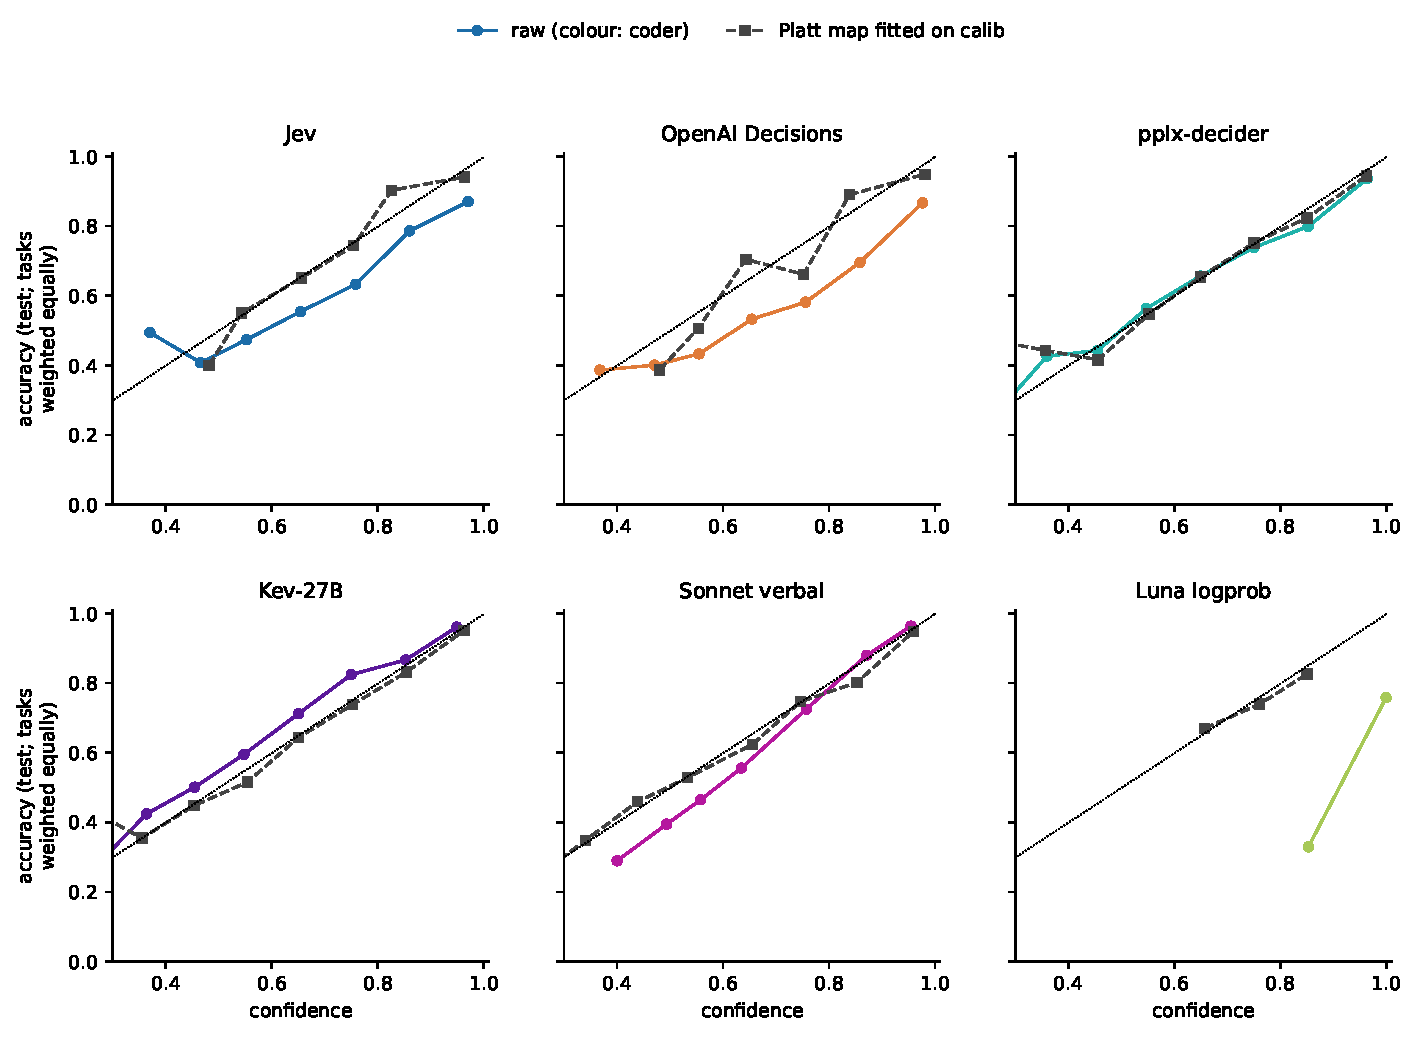
\includegraphics[width=0.85\linewidth]{fig03_reliability.pdf}
  \caption{EQ1: reliability on the test split before (coloured) and after (dashed grey) a Platt map fitted per task on the
  calibration split, for four decision models, Sonnet's verbalized confidence and Luna's token probabilities. Tasks are weighted equally; bins with fewer than 20 decisions are omitted.}
  \label{fig:reliability}
\end{figure}
\begin{table}[t]
\centering
\small
\caption{EQ1 (exploratory): recalibration and the fixed rule 'accept if confidence $\geq$ 0.95' (pooled)}
\label{tab:tab07_triage_rules}
\par\textit{A. Expected calibration error, raw and after recalibration}\par\smallskip
\begin{adjustbox}{max width=\linewidth}
\begin{tabular}{lrrrr}
\toprule
signal & ECE raw & ECE Platt & ECE isotonic & \makecell[br]{ECE \\{} temperature} \\
\midrule
Jev & 0.120 & 0.038 & 0.040 & 0.120 \\
OpenAI Decisions & 0.122 & 0.073 & 0.042 & 0.098 \\
Clef (27B) & 0.055 & 0.041 & 0.045 & 0.054 \\
Clef-flash (9B) & 0.065 & 0.043 & 0.035 & 0.051 \\
pplx-decider & 0.052 & 0.043 & 0.048 & 0.047 \\
Kev-9B & 0.100 & 0.041 & 0.053 & 0.069 \\
Kev-27B & 0.073 & 0.032 & 0.037 & 0.029 \\
Luna verbal & 0.180 & 0.047 & 0.040 & 0.059 \\
Haiku verbal & 0.154 & 0.045 & 0.035 & 0.075 \\
gpt-oss verbal & 0.204 & 0.056 & 0.038 & 0.075 \\
Qwen3.5-9B verbal & 0.303 & 0.045 & 0.037 & 0.099 \\
Luna logprob & 0.243 & 0.038 & 0.039 & 0.106 \\
gpt-oss logprob & 0.284 & 0.040 & 0.045 & 0.033 \\
Qwen3.5-9B logprob & 0.334 & 0.052 & 0.054 & 0.060 \\
Sonnet verbal & 0.051 & 0.034 & 0.039 & 0.053 \\
Qwen3.8-2.4T verbal & 0.102 & 0.060 & 0.061 & 0.091 \\
\bottomrule
\end{tabular}
\end{adjustbox}
\medskip
\par\textit{B. Error ranking, and the fixed rule 'accept if confidence $\geq$ 0.95' applied to raw confidence}\par\smallskip
\begin{adjustbox}{max width=\linewidth}
\begin{tabular}{lrrrr}
\toprule
signal & \makecell[br]{error AUROC \\{} raw} & \makecell[br]{error AUROC \\{} Platt} & \makecell[br]{share accepted \\{} by '$\geq$ 0.95'} & its error \\
\midrule
Jev & 0.756 & 0.756 & 0.364 & 0.121 \\
OpenAI Decisions & 0.736 & 0.736 & 0.498 & 0.115 \\
Clef (27B) & 0.721 & 0.721 & 0.081 & 0.007 \\
Clef-flash (9B) & 0.712 & 0.712 & 0.043 & 0.001 \\
pplx-decider & 0.764 & 0.764 & 0.281 & 0.041 \\
Kev-9B & 0.694 & 0.694 & 0.041 & 0.032 \\
Kev-27B & 0.788 & 0.788 & 0.155 & 0.034 \\
Luna verbal & 0.741 & 0.741 & 0.635 & 0.139 \\
Haiku verbal & 0.783 & 0.783 & 0.310 & 0.044 \\
gpt-oss verbal & 0.727 & 0.727 & 0.523 & 0.120 \\
Qwen3.5-9B verbal & 0.646 & 0.646 & 0.966 & 0.331 \\
Luna logprob & 0.558 & 0.556 & 0.994 & 0.241 \\
gpt-oss logprob & 0.558 & 0.539 & 0.998 & 0.285 \\
Qwen3.5-9B logprob & 0.684 & 0.684 & 0.984 & 0.334 \\
Sonnet verbal & 0.801 & 0.801 & 0.225 & 0.021 \\
Qwen3.8-2.4T verbal & 0.802 & 0.802 & 0.259 & 0.020 \\
\bottomrule
\end{tabular}
\end{adjustbox}
\par\smallskip\footnotesize\raggedright Maps fitted per task on calib. Platt and isotonic maps act on the decision's confidence; temperature scaling acts on the full distribution and is sensitive to how exact 0s and 1s are floored (Table~\ref{tab:tab24_temperature_floor}; here 1e-12). Errors are among accepted test decisions.
\end{table}

\begin{table}[t]
\centering
\small
\caption{Temperature scaling and per-code maps depend on how exact 0s and 1s are floored before taking logarithms (pooled)}
\label{tab:tab24_temperature_floor}
\par\textit{A. ECE}\par\smallskip
\begin{adjustbox}{max width=\linewidth}
\begin{tabular}{lrrr}
\toprule
signal & raw & \makecell[br]{temperature, \\{} floor 1e-4} & \makecell[br]{temperature, \\{} floor 1e-12} \\
\midrule
Jev & 0.120 & 0.046 & 0.120 \\
Kev-27B & 0.073 & 0.029 & 0.029 \\
Luna logprob & 0.243 & 0.040 & 0.106 \\
OpenAI Decisions & 0.122 & 0.040 & 0.098 \\
gpt-oss logprob & 0.284 & 0.033 & 0.033 \\
Qwen3.5-9B logprob & 0.334 & 0.055 & 0.060 \\
Sonnet verbal & 0.051 & 0.053 & 0.053 \\
\bottomrule
\end{tabular}
\end{adjustbox}
\medskip
\par\textit{B. Error AUROC}\par\smallskip
\begin{adjustbox}{max width=\linewidth}
\begin{tabular}{lrrrrr}
\toprule
signal & raw & \makecell[br]{temperature, \\{} floor 1e-4} & \makecell[br]{temperature, \\{} floor 1e-12} & \makecell[br]{per-code \\{} Platt, floor \\{} 1e-4} & \makecell[br]{per-code \\{} Platt, floor \\{} 1e-12} \\
\midrule
Jev & 0.756 & 0.757 & 0.749 & 0.809 & 0.797 \\
Kev-27B & 0.788 & 0.788 & 0.788 & 0.814 & 0.814 \\
Luna logprob & 0.558 & 0.489 & 0.579 & 0.670 & 0.671 \\
OpenAI Decisions & 0.736 & 0.735 & 0.735 & 0.785 & 0.771 \\
gpt-oss logprob & 0.558 & 0.495 & 0.542 & 0.698 & 0.717 \\
Qwen3.5-9B logprob & 0.684 & 0.665 & 0.666 & 0.733 & 0.757 \\
Sonnet verbal & 0.801 & 0.802 & 0.802 & 0.826 & 0.826 \\
\bottomrule
\end{tabular}
\end{adjustbox}
\par\smallskip\footnotesize\raggedright One temperature per task, fitted by weighted log-loss on calib. A task-level Platt or isotonic map is monotone and leaves error ranking unchanged at any floor; per-code Platt maps (EQ3) are not monotone across codes, so the floor changes their ranking for coders that return exact 0s and 1s.
\end{table}

\FloatBarrier

\subsection{EQ2: threshold rules and the cost of a guarantee}
These analyses test whether each threshold rule keeps its 5\% target and what a valid guarantee costs (\S\ref{sec:eq2}). The
re-split tables repeat the random calibration/test split 500 times per task: the naive rule exceeds 5\% in about half of
them on MFRC and LTT on decisions in more than the nominal 5\%, while corpus LTT never does. The budget curves and the single-threshold variant show how
much hand-coding a guarantee needs on MFRC. The simulation checks each rule against a known true risk under correlated
errors, and the feasibility and utterance-sampling tables show why dialogue certifies nothing under whole-transcript
sampling, and why sampling single utterances removes that obstacle yet still yields almost no certificates for the real
coders.

\begin{table}[t]
\centering
\small
\caption{EQ2 (exploratory): threshold rules at a 5\% target (percent)}
\label{tab:tab07c_threshold_rules}
\par\textit{A. Frozen split, pooled over tasks}\par\smallskip
\begin{adjustbox}{max width=\linewidth}
\begin{tabular}{lrrrrr}
\toprule
signal & \makecell[br]{naive: \\{} accepted} & naive: error & \makecell[br]{corpus LTT: \\{} accepted} & \makecell[br]{corpus LTT: \\{} error} & \makecell[br]{oracle: \\{} accepted} \\
\midrule
Jev & 32.9 & 6.8 & 12.0 & 1.6 & 16.3 \\
OpenAI Decisions & 22.7 & 4.7 & 0.0 & -- & 17.8 \\
Clef (27B) & 24.0 & 5.8 & 16.5 & 3.0 & 20.3 \\
Clef-flash (9B) & 25.4 & 7.0 & 15.6 & 2.7 & 20.7 \\
pplx-decider & 40.8 & 7.5 & 15.4 & 2.3 & 32.1 \\
Kev-9B & 23.9 & 6.3 & 13.4 & 2.4 & 19.2 \\
Kev-27B & 44.2 & 7.0 & 15.3 & 2.1 & 37.2 \\
Luna verbal & 20.2 & 4.6 & 12.8 & 2.2 & 16.2 \\
Haiku verbal & 16.1 & 3.2 & 13.2 & 1.7 & 16.8 \\
gpt-oss verbal & 22.1 & 5.6 & 0.0 & -- & 20.6 \\
Qwen3.5-9B verbal & 3.4 & 11.4 & 0.0 & -- & 0.0 \\
Luna logprob & 0.0 & -- & 0.0 & -- & 11.8 \\
gpt-oss logprob & 1.2 & 29.7 & 0.0 & -- & 0.0 \\
Qwen3.5-9B logprob & 9.3 & 7.9 & 0.0 & -- & 8.2 \\
Sonnet verbal & 43.4 & 6.2 & 16.5 & 2.5 & 40.1 \\
Qwen3.8-2.4T verbal & 37.9 & 4.3 & 0.0 & -- & 38.0 \\
\bottomrule
\end{tabular}
\end{adjustbox}
\medskip
\par\textit{B. MFRC: share of re-splits with held-out error above 5\%, and corpus LTT with per-code maps}\par\smallskip
\begin{adjustbox}{max width=\linewidth}
\begin{tabular}{lrrrrr}
\toprule
signal & naive & \makecell[br]{LTT on \\{} decisions} & \makecell[br]{LTT on i.i.d. \\{} clusters} & corpus LTT & \makecell[br]{per-code maps, \\{} corpus LTT: \\{} accepted} \\
\midrule
Jev & 49.4 & 6.8 & 0.0 & 0.0 & 0.0 \\
OpenAI Decisions & 28.0 & 5.8 & 0.0 & 0.0 & 0.0 \\
Clef (27B) & 47.0 & 8.4 & 0.0 & 0.0 & 75.4 \\
Clef-flash (9B) & 51.8 & 8.4 & 0.0 & 0.0 & 65.5 \\
pplx-decider & 50.0 & 11.2 & 0.0 & 0.0 & 72.0 \\
Kev-9B & 52.4 & 9.0 & 0.0 & 0.0 & 0.0 \\
Kev-27B & 47.0 & 9.2 & 0.0 & 0.0 & 0.0 \\
Luna verbal & 5.2 & 0.0 & 0.0 & 0.0 & 0.0 \\
Haiku verbal & 19.4 & 6.0 & 0.0 & 0.0 & 0.0 \\
gpt-oss verbal & 0.0 & 0.0 & 0.0 & 0.0 & 0.0 \\
Qwen3.5-9B verbal & 0.0 & 0.0 & 0.0 & 0.0 & 0.0 \\
Luna logprob & 0.0 & 0.0 & 0.0 & 0.0 & 0.0 \\
gpt-oss logprob & 15.2 & 0.0 & 0.0 & 0.0 & 0.0 \\
Qwen3.5-9B logprob & 47.2 & 5.2 & 0.0 & 0.0 & 0.0 \\
Sonnet verbal & 6.0 & 0.0 & 0.0 & 0.0 & 68.9 \\
Qwen3.8-2.4T verbal & 5.2 & 0.6 & 0.0 & 0.0 & 0.0 \\
\bottomrule
\end{tabular}
\end{adjustbox}
\par\smallskip\footnotesize\raggedright Panel A: frozen split, equal-weight means over the five tasks; oracle: fitted on test. Panel B: 500 random cluster re-splits of MFRC; for corpus LTT each test split is the uncoded remainder of its re-split, so exceedance there is a direct check of its guarantee. Per-code maps are fitted on half of the calib clusters, frozen, certified on the other half and applied unchanged to test.
\end{table}

\begin{table}[t]
\centering
\small
\caption{Naive rule and LTT on decisions by task over 500 cluster re-splits (percent)}
\label{tab:tab07b_resplits_by_task}
\begin{adjustbox}{max width=\linewidth}
\begin{tabular}{llrrrrrr}
\toprule
signal & task & \makecell[br]{naive: \\{} accepted} & \makecell[br]{naive: none \\{} accepted} & \makecell[br]{naive: \\{} error > 5\%} & \makecell[br]{LTT on \\{} decisions: \\{} accepted} & \makecell[br]{LTT on \\{} decisions: \\{} none \\{} accepted} & \makecell[br]{LTT on \\{} decisions: \\{} error > 5\%} \\
\midrule
Clef (27B) & AnnoMI client & 7.3 & 5.0 & 73.8 & 0.0 & 100.0 & 0.0 \\
Clef (27B) & AnnoMI therapist & 18.8 & 0.0 & 63.6 & 0.2 & 99.4 & 0.6 \\
Clef (27B) & MFRC & 90.2 & 0.0 & 47.0 & 88.3 & 0.0 & 8.4 \\
Clef (27B) & TalkMoves student & 1.4 & 0.2 & 65.4 & 0.0 & 100.0 & 0.0 \\
Clef (27B) & TalkMoves teacher & 0.6 & 0.8 & 67.8 & 0.0 & 100.0 & 0.0 \\
Clef-flash (9B) & AnnoMI client & 11.5 & 1.2 & 84.8 & 0.0 & 100.0 & 0.0 \\
Clef-flash (9B) & AnnoMI therapist & 10.8 & 8.2 & 56.4 & 0.0 & 100.0 & 0.0 \\
Clef-flash (9B) & MFRC & 89.8 & 0.0 & 51.8 & 87.1 & 0.0 & 8.4 \\
Clef-flash (9B) & TalkMoves student & 2.4 & 0.0 & 33.2 & 0.0 & 100.0 & 0.0 \\
Clef-flash (9B) & TalkMoves teacher & 0.4 & 6.6 & 53.2 & 0.0 & 100.0 & 0.0 \\
Jev & AnnoMI client & 3.1 & 91.0 & 9.0 & 0.0 & 100.0 & 0.0 \\
Jev & AnnoMI therapist & 18.0 & 62.8 & 37.2 & 0.1 & 99.8 & 0.2 \\
Jev & MFRC & 80.8 & 0.0 & 49.4 & 78.3 & 0.0 & 6.8 \\
Jev & TalkMoves student & 1.7 & 85.0 & 15.0 & 0.0 & 100.0 & 0.0 \\
Jev & TalkMoves teacher & 2.5 & 81.0 & 19.0 & 0.0 & 100.0 & 0.0 \\
Kev-27B & AnnoMI client & 15.6 & 0.2 & 70.2 & 0.0 & 100.0 & 0.0 \\
Kev-27B & AnnoMI therapist & 51.9 & 0.0 & 41.8 & 12.4 & 68.0 & 2.0 \\
Kev-27B & MFRC & 94.0 & 0.0 & 47.0 & 91.7 & 0.0 & 9.2 \\
Kev-27B & TalkMoves student & 20.3 & 0.0 & 62.8 & 0.0 & 100.0 & 0.0 \\
Kev-27B & TalkMoves teacher & 21.9 & 0.6 & 72.2 & 0.0 & 100.0 & 0.0 \\
Kev-9B & AnnoMI client & 2.8 & 0.4 & 68.8 & 0.0 & 100.0 & 0.0 \\
Kev-9B & AnnoMI therapist & 14.2 & 0.0 & 79.8 & 0.1 & 99.6 & 0.4 \\
Kev-9B & MFRC & 87.8 & 0.0 & 52.4 & 56.8 & 16.0 & 9.0 \\
Kev-9B & TalkMoves student & 0.2 & 67.0 & 33.0 & 0.0 & 100.0 & 0.0 \\
Kev-9B & TalkMoves teacher & 0.4 & 5.6 & 41.6 & 0.0 & 100.0 & 0.0 \\
OpenAI Decisions & AnnoMI client & 1.8 & 91.8 & 8.2 & 0.0 & 100.0 & 0.0 \\
OpenAI Decisions & AnnoMI therapist & 32.1 & 18.8 & 51.2 & 1.4 & 96.8 & 3.2 \\
OpenAI Decisions & MFRC & 74.3 & 0.0 & 28.0 & 69.6 & 0.0 & 5.8 \\
OpenAI Decisions & TalkMoves student & 0.9 & 30.6 & 69.4 & 0.0 & 100.0 & 0.0 \\
OpenAI Decisions & TalkMoves teacher & 0.1 & 99.6 & 0.4 & 0.0 & 100.0 & 0.0 \\
pplx-decider & AnnoMI client & 17.3 & 0.0 & 65.0 & 0.0 & 100.0 & 0.0 \\
pplx-decider & AnnoMI therapist & 58.8 & 0.0 & 53.4 & 9.1 & 80.0 & 2.6 \\
pplx-decider & MFRC & 91.5 & 0.0 & 50.0 & 89.2 & 0.0 & 11.2 \\
pplx-decider & TalkMoves student & 13.1 & 0.0 & 52.0 & 0.0 & 100.0 & 0.0 \\
pplx-decider & TalkMoves teacher & 3.4 & 44.0 & 56.0 & 0.0 & 100.0 & 0.0 \\
Sonnet verbal & AnnoMI client & 12.7 & 0.2 & 49.2 & 0.2 & 99.2 & 0.8 \\
Sonnet verbal & AnnoMI therapist & 56.0 & 0.0 & 38.6 & 7.7 & 83.8 & 3.0 \\
Sonnet verbal & MFRC & 89.8 & 0.0 & 6.0 & 88.9 & 0.0 & 0.0 \\
Sonnet verbal & TalkMoves student & 11.6 & 10.6 & 62.0 & 0.0 & 100.0 & 0.0 \\
Sonnet verbal & TalkMoves teacher & 39.0 & 0.0 & 39.2 & 1.8 & 95.4 & 4.2 \\
\bottomrule
\end{tabular}
\end{adjustbox}
\par\smallskip\footnotesize\raggedright Accepted: mean share of test decisions accepted; none accepted: share of re-splits accepting nothing; error > 5\%: share of re-splits whose held-out error exceeds 5\%. A re-split that accepts nothing cannot exceed 5\%; read exceedance with acceptance.
\end{table}

\begin{table}[t]
\centering
\small
\caption{LTT on i.i.d. clusters and corpus LTT by task over 500 cluster re-splits (percent)}
\label{tab:tab07d_resplits_guaranteed}
\begin{adjustbox}{max width=\linewidth}
\begin{tabular}{llrrrrrr}
\toprule
signal & task & \makecell[br]{i.i.d.-cluster \\{} LTT: \\{} accepted} & \makecell[br]{i.i.d.-cluster \\{} LTT: none \\{} accepted} & \makecell[br]{i.i.d.-cluster \\{} LTT: error \\{} > 5\%} & \makecell[br]{corpus LTT: \\{} accepted} & \makecell[br]{corpus LTT: \\{} none \\{} accepted} & \makecell[br]{corpus LTT: \\{} error > 5\%} \\
\midrule
Clef (27B) & AnnoMI client & 0.0 & 100.0 & 0.0 & 0.0 & 100.0 & 0.0 \\
Clef (27B) & AnnoMI therapist & 0.0 & 100.0 & 0.0 & 0.0 & 100.0 & 0.0 \\
Clef (27B) & MFRC & 82.3 & 0.0 & 0.0 & 81.0 & 0.0 & 0.0 \\
Clef (27B) & TalkMoves student & 0.0 & 100.0 & 0.0 & 0.0 & 100.0 & 0.0 \\
Clef (27B) & TalkMoves teacher & 0.0 & 100.0 & 0.0 & 0.0 & 100.0 & 0.0 \\
Clef-flash (9B) & AnnoMI client & 0.0 & 100.0 & 0.0 & 0.0 & 100.0 & 0.0 \\
Clef-flash (9B) & AnnoMI therapist & 0.0 & 100.0 & 0.0 & 0.0 & 100.0 & 0.0 \\
Clef-flash (9B) & MFRC & 79.2 & 0.0 & 0.0 & 77.5 & 0.0 & 0.0 \\
Clef-flash (9B) & TalkMoves student & 0.0 & 100.0 & 0.0 & 0.0 & 100.0 & 0.0 \\
Clef-flash (9B) & TalkMoves teacher & 0.0 & 100.0 & 0.0 & 0.0 & 100.0 & 0.0 \\
Jev & AnnoMI client & 0.0 & 100.0 & 0.0 & 0.0 & 100.0 & 0.0 \\
Jev & AnnoMI therapist & 0.0 & 100.0 & 0.0 & 0.0 & 100.0 & 0.0 \\
Jev & MFRC & 69.7 & 0.0 & 0.0 & 67.5 & 0.0 & 0.0 \\
Jev & TalkMoves student & 0.0 & 100.0 & 0.0 & 0.0 & 100.0 & 0.0 \\
Jev & TalkMoves teacher & 0.0 & 100.0 & 0.0 & 0.0 & 100.0 & 0.0 \\
Kev-27B & AnnoMI client & 0.0 & 100.0 & 0.0 & 0.0 & 100.0 & 0.0 \\
Kev-27B & AnnoMI therapist & 0.0 & 100.0 & 0.0 & 0.0 & 100.0 & 0.0 \\
Kev-27B & MFRC & 84.8 & 0.0 & 0.0 & 82.4 & 0.0 & 0.0 \\
Kev-27B & TalkMoves student & 0.0 & 100.0 & 0.0 & 0.0 & 100.0 & 0.0 \\
Kev-27B & TalkMoves teacher & 0.0 & 100.0 & 0.0 & 0.0 & 100.0 & 0.0 \\
Kev-9B & AnnoMI client & 0.0 & 100.0 & 0.0 & 0.0 & 100.0 & 0.0 \\
Kev-9B & AnnoMI therapist & 0.0 & 100.0 & 0.0 & 0.0 & 100.0 & 0.0 \\
Kev-9B & MFRC & 75.9 & 0.0 & 0.0 & 72.3 & 0.6 & 0.0 \\
Kev-9B & TalkMoves student & 0.0 & 100.0 & 0.0 & 0.0 & 100.0 & 0.0 \\
Kev-9B & TalkMoves teacher & 0.0 & 100.0 & 0.0 & 0.0 & 100.0 & 0.0 \\
OpenAI Decisions & AnnoMI client & 0.0 & 100.0 & 0.0 & 0.0 & 100.0 & 0.0 \\
OpenAI Decisions & AnnoMI therapist & 0.0 & 100.0 & 0.0 & 0.0 & 100.0 & 0.0 \\
OpenAI Decisions & MFRC & 14.8 & 67.0 & 0.0 & 0.4 & 99.0 & 0.0 \\
OpenAI Decisions & TalkMoves student & 0.0 & 100.0 & 0.0 & 0.0 & 100.0 & 0.0 \\
OpenAI Decisions & TalkMoves teacher & 0.0 & 100.0 & 0.0 & 0.0 & 100.0 & 0.0 \\
pplx-decider & AnnoMI client & 0.0 & 100.0 & 0.0 & 0.0 & 100.0 & 0.0 \\
pplx-decider & AnnoMI therapist & 0.0 & 100.0 & 0.0 & 0.0 & 100.0 & 0.0 \\
pplx-decider & MFRC & 82.7 & 0.0 & 0.0 & 81.1 & 0.0 & 0.0 \\
pplx-decider & TalkMoves student & 0.0 & 100.0 & 0.0 & 0.0 & 100.0 & 0.0 \\
pplx-decider & TalkMoves teacher & 0.0 & 100.0 & 0.0 & 0.0 & 100.0 & 0.0 \\
Sonnet verbal & AnnoMI client & 0.0 & 100.0 & 0.0 & 0.0 & 100.0 & 0.0 \\
Sonnet verbal & AnnoMI therapist & 0.0 & 100.0 & 0.0 & 0.0 & 100.0 & 0.0 \\
Sonnet verbal & MFRC & 85.4 & 0.0 & 0.0 & 84.5 & 0.0 & 0.0 \\
Sonnet verbal & TalkMoves student & 0.0 & 100.0 & 0.0 & 0.0 & 100.0 & 0.0 \\
Sonnet verbal & TalkMoves teacher & 0.0 & 100.0 & 0.0 & 0.0 & 100.0 & 0.0 \\
\bottomrule
\end{tabular}
\end{adjustbox}
\par\smallskip\footnotesize\raggedright Accepted: mean share of test decisions accepted; none accepted: share of re-splits accepting nothing; error > 5\%: share of re-splits whose held-out error exceeds 5\%. A re-split that accepts nothing cannot exceed 5\%; read exceedance with acceptance.
\end{table}

\begin{figure}[htbp]
  \centering
  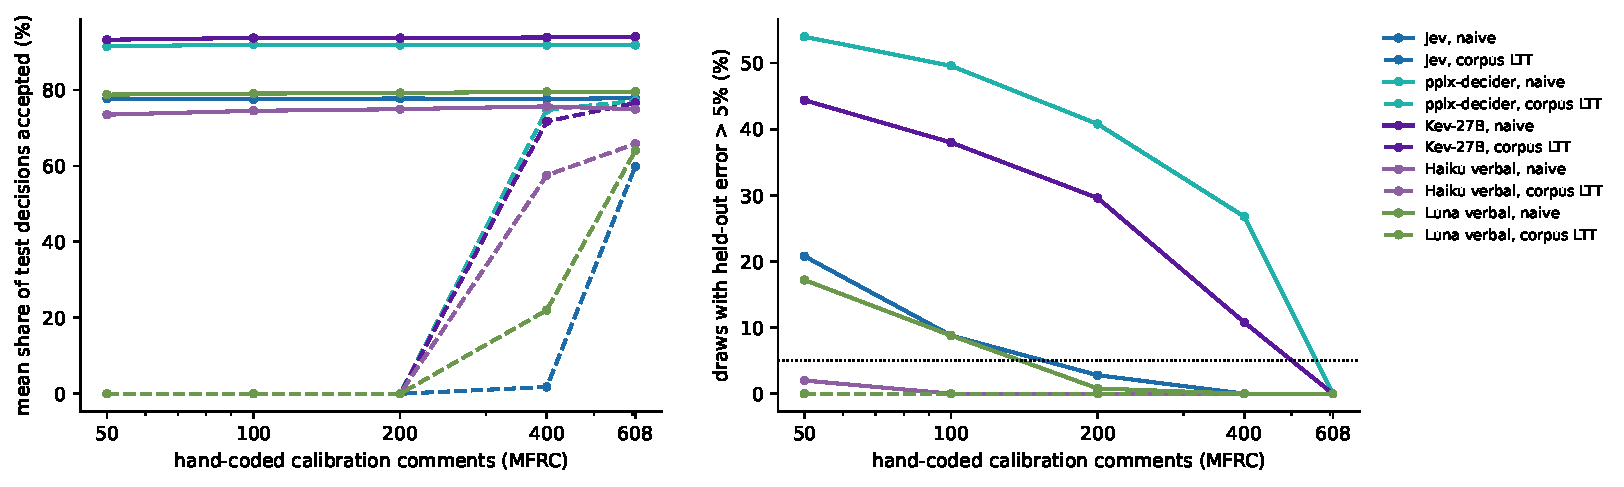
\includegraphics[width=\linewidth]{fig06_calibration_budget.pdf}
  \caption{EQ2: calibration budget on MFRC. Left: mean share of test decisions accepted; right: share of draws whose held-out
  error exceeds 5\%, when only $n$ randomly drawn comments are hand-coded (250 draws; 608 is the full calibration split).
  Solid: naive rule; dashed: corpus LTT. Corpus LTT certifies nothing for any plotted coder with 200 or fewer comments, and 2\%
  (Jev) to 75\% (pplx-decider) with 400. For each draw the corpus is the drawn comments plus the test split, whose decisions are
  the ones scored. The dialogue tasks are omitted: with whole transcripts hand-coded, corpus LTT certifies nothing there.}
  \label{fig:budget}
\end{figure}
\begin{table}[t]
\centering
\small
\caption{MFRC: corpus LTT over the 16-threshold grid vs one threshold fixed in advance (0.95)}
\label{tab:tab23_ltt_single_threshold}
\begin{adjustbox}{max width=\linewidth}
\begin{tabular}{lrrrr}
\toprule
signal & \makecell[br]{grid of 16: \\{} accepted} & error & \makecell[br]{one threshold \\{} (0.95): \\{} accepted} & error \\
\midrule
Jev & 0.598 & 0.016 & 0.170 & 0.006 \\
OpenAI Decisions & 0.000 & -- & 0.000 & -- \\
Clef (27B) & 0.823 & 0.030 & 0.365 & 0.001 \\
Clef-flash (9B) & 0.779 & 0.027 & 0.213 & 0.001 \\
pplx-decider & 0.771 & 0.023 & 0.656 & 0.013 \\
Kev-9B & 0.671 & 0.024 & 0.176 & 0.010 \\
Kev-27B & 0.766 & 0.021 & 0.294 & 0.003 \\
Luna verbal & 0.640 & 0.022 & 0.745 & 0.034 \\
Haiku verbal & 0.658 & 0.017 & 0.549 & 0.008 \\
gpt-oss verbal & 0.000 & -- & 0.718 & 0.026 \\
Sonnet verbal & 0.827 & 0.025 & 0.624 & 0.007 \\
\bottomrule
\end{tabular}
\end{adjustbox}
\par\smallskip\footnotesize\raggedright On the four dialogue tasks, with the original whole-cluster split, neither version certifies anything for any coder.
\end{table}

\begin{table}[t]
\centering
\small
\caption{LTT on synthetic clustered corpora (300 simulations per row, 30\% of clusters hand-coded, $\delta$ = 0.05)}
\label{tab:tab20_ltt_simulation}
\begin{adjustbox}{max width=\linewidth}
\begin{tabular}{rrrrlrrr}
\toprule
\makecell[br]{clusters in \\{} corpus} & \makecell[br]{decisions per \\{} cluster} & \makecell[br]{copula \\{} loading} & \makecell[br]{within-cluster \\{} error \\{} correlation} & LTT on & \makecell[br]{P(remainder \\{} risk > 5\%)} & \makecell[br]{P(population \\{} risk > 5\%)} & \makecell[br]{mean share \\{} accepted} \\
\midrule
2000 & 8 & 0.000 & -0.002 & decisions & 0.103 & 0.057 & 0.775 \\
2000 & 8 & 0.000 & -0.002 & i.i.d. clusters & 0.000 & 0.000 & 0.522 \\
2000 & 8 & 0.000 & -0.002 & corpus & 0.000 & 0.000 & 0.289 \\
2000 & 8 & 0.500 & 0.070 & decisions & 0.113 & 0.067 & 0.772 \\
2000 & 8 & 0.500 & 0.070 & i.i.d. clusters & 0.000 & 0.000 & 0.477 \\
2000 & 8 & 0.500 & 0.070 & corpus & 0.000 & 0.000 & 0.249 \\
2000 & 8 & 0.900 & 0.364 & decisions & 0.163 & 0.137 & 0.763 \\
2000 & 8 & 0.900 & 0.364 & i.i.d. clusters & 0.003 & 0.000 & 0.362 \\
2000 & 8 & 0.900 & 0.364 & corpus & 0.003 & 0.000 & 0.146 \\
400 & 10 & 0.900 & 0.329 & decisions & 0.193 & 0.180 & 0.616 \\
400 & 10 & 0.900 & 0.329 & i.i.d. clusters & 0.000 & 0.000 & 0.000 \\
400 & 10 & 0.900 & 0.329 & corpus & 0.000 & 0.000 & 0.000 \\
170 & 30 & 0.900 & 0.328 & decisions & 0.297 & 0.313 & 0.656 \\
170 & 30 & 0.900 & 0.328 & i.i.d. clusters & 0.000 & 0.000 & 0.000 \\
170 & 30 & 0.900 & 0.328 & corpus & 0.000 & 0.000 & 0.000 \\
\bottomrule
\end{tabular}
\end{adjustbox}
\par\smallskip\footnotesize\raggedright Calibrated confidence conf = 1 -- 0.5·Beta(1, 6); errors correlated within a cluster through a Gaussian copula (the loading is not the error correlation, which is shown). Remainder: the uncoded clusters of the corpus; population: closed form. The best threshold with population risk $\leq$ 5\% accepts 0.841 of decisions.
\end{table}

\begin{table}[t]
\centering
\small
\caption{Our corpus LTT procedure: hand-coded units needed before it certifies a coder that is never wrong}
\label{tab:tab21_ltt_feasibility}
\par\textit{A. Grid of 16 thresholds (as used throughout)}\par\smallskip
\begin{adjustbox}{max width=\linewidth}
\begin{tabular}{llrrlll}
\toprule
task & \makecell[bl]{sampling \\{} unit} & \makecell[br]{units in \\{} corpus} & \makecell[br]{mean unit \\{} weight / B} & \makecell[bl]{frozen split \\{} certifies it} & lower bound & \makecell[bl]{our \\{} procedure \\{} (median)} \\
\midrule
MFRC & comment & 2000 & 1.00 & yes & 119 & 123 \\
AnnoMI client & transcript & 128 & 0.12 & no & unreachable & not reached \\
AnnoMI client & utterance & 1500 & 0.85 & -- & 119 & 146.5 \\
AnnoMI therapist & transcript & 132 & 0.13 & no & unreachable & not reached \\
AnnoMI therapist & utterance & 1500 & 0.87 & -- & 119 & 145 \\
TalkMoves teacher & lesson & 444 & 0.27 & no & 388 & not reached \\
TalkMoves teacher & sentence & 1500 & 0.78 & -- & 119 & 163 \\
TalkMoves student & lesson & 436 & 0.08 & no & unreachable & not reached \\
TalkMoves student & sentence & 1500 & 0.90 & -- & 119 & 139 \\
\bottomrule
\end{tabular}
\end{adjustbox}
\medskip
\par\textit{B. One threshold fixed in advance (0.95)}\par\smallskip
\begin{adjustbox}{max width=\linewidth}
\begin{tabular}{llrll}
\toprule
task & \makecell[bl]{sampling \\{} unit} & \makecell[br]{units in \\{} corpus} & lower bound & \makecell[bl]{our \\{} procedure \\{} (median)} \\
\midrule
MFRC & comment & 2000 & 62 & 64 \\
AnnoMI client & transcript & 128 & unreachable & not reached \\
AnnoMI client & utterance & 1500 & 62 & 75 \\
AnnoMI therapist & transcript & 132 & unreachable & not reached \\
AnnoMI therapist & utterance & 1500 & 62 & 75 \\
TalkMoves teacher & lesson & 444 & 114 & not reached \\
TalkMoves teacher & sentence & 1500 & 62 & 81.5 \\
TalkMoves student & lesson & 436 & unreachable & not reached \\
TalkMoves student & sentence & 1500 & 62 & 70.5 \\
\bottomrule
\end{tabular}
\end{adjustbox}
\par\smallskip\footnotesize\raggedright B: the largest unit's weight. Lower bound: a necessary number over every set of hand-coded units and every visiting order (each unit's bet can multiply the evidence by at most 1 + 0.05 $\times$ its weight / B, and certification needs a factor of 320 with the grid, 20 with one threshold); fewer units cannot suffice, and reaching the bound does not guarantee certification. Unreachable: not reached even with every unit but one hand-coded. Our procedure: median number of units at which it first certifies, over 20 random hand-coding sequences (a description of typical runs, not a bound). Transcripts and lessons are the units of our splits; utterances and sentences drawn at random are an alternative design.
\end{table}

\begin{table}[t]
\centering
\small
\caption{Dialogue tasks under a different hand-coding design: corpus LTT with single utterances or sentences drawn at random (exploratory; 200 re-splits, 30\% hand-coded)}
\label{tab:tab21b_utterance_sampling}
\par\textit{A. Corpus LTT: mean share of the remainder's decisions accepted (percent; re-splits with no certificate count as 0)}\par\smallskip
\begin{adjustbox}{max width=\linewidth}
\begin{tabular}{lrrrr}
\toprule
signal & \makecell[br]{AnnoMI \\{} client} & \makecell[br]{AnnoMI \\{} therapist} & \makecell[br]{TalkMoves \\{} teacher} & \makecell[br]{TalkMoves \\{} student} \\
\midrule
Jev & 0.0 & 0.0 & 0.0 & 0.0 \\
OpenAI Decisions & 0.0 & 0.0 & 0.0 & 0.0 \\
Clef (27B) & 0.0 & 0.0 & 0.0 & 0.0 \\
Clef-flash (9B) & 0.0 & 0.0 & 0.0 & 0.0 \\
pplx-decider & 0.0 & 0.4 & 0.0 & 0.0 \\
Kev-9B & 0.0 & 0.0 & 0.0 & 0.0 \\
Kev-27B & 0.0 & 0.2 & 0.0 & 0.0 \\
Luna verbal & 0.0 & 0.0 & 0.0 & 0.0 \\
Haiku verbal & 0.0 & 0.0 & 0.0 & 0.0 \\
gpt-oss verbal & 0.0 & 0.0 & 0.0 & 0.0 \\
Sonnet verbal & 0.0 & 0.0 & 0.0 & 0.0 \\
\bottomrule
\end{tabular}
\end{adjustbox}
\medskip
\par\textit{B. Corpus LTT: re-splits with any certified threshold}\par\smallskip
\begin{adjustbox}{max width=\linewidth}
\begin{tabular}{lllll}
\toprule
signal & \makecell[bl]{AnnoMI \\{} client} & \makecell[bl]{AnnoMI \\{} therapist} & \makecell[bl]{TalkMoves \\{} teacher} & \makecell[bl]{TalkMoves \\{} student} \\
\midrule
Jev & 0 of 200 & 0 of 200 & 0 of 200 & 0 of 200 \\
OpenAI Decisions & 0 of 200 & 0 of 200 & 0 of 200 & 0 of 200 \\
Clef (27B) & 0 of 200 & 0 of 200 & 0 of 200 & 0 of 200 \\
Clef-flash (9B) & 0 of 200 & 0 of 200 & 0 of 200 & 0 of 200 \\
pplx-decider & 0 of 200 & 2 of 200 & 0 of 200 & 0 of 200 \\
Kev-9B & 0 of 200 & 0 of 200 & 0 of 200 & 0 of 200 \\
Kev-27B & 0 of 200 & 1 of 200 & 0 of 200 & 0 of 200 \\
Luna verbal & 0 of 200 & 0 of 200 & 0 of 200 & 0 of 200 \\
Haiku verbal & 0 of 200 & 0 of 200 & 0 of 200 & 0 of 200 \\
gpt-oss verbal & 0 of 200 & 0 of 200 & 0 of 200 & 0 of 200 \\
Sonnet verbal & 0 of 200 & 0 of 200 & 0 of 200 & 0 of 200 \\
\bottomrule
\end{tabular}
\end{adjustbox}
\medskip
\par\textit{C. Naive rule: share of re-splits whose accepted decisions exceed 5\% error (percent)}\par\smallskip
\begin{adjustbox}{max width=\linewidth}
\begin{tabular}{lrrrr}
\toprule
signal & \makecell[br]{AnnoMI \\{} client} & \makecell[br]{AnnoMI \\{} therapist} & \makecell[br]{TalkMoves \\{} teacher} & \makecell[br]{TalkMoves \\{} student} \\
\midrule
Jev & 1.0 & 35.0 & 15.0 & 23.0 \\
OpenAI Decisions & 6.0 & 45.5 & 1.0 & 67.0 \\
Clef (27B) & 70.5 & 67.5 & 77.0 & 67.5 \\
Clef-flash (9B) & 74.0 & 58.5 & 55.5 & 38.0 \\
pplx-decider & 59.0 & 51.5 & 58.0 & 50.0 \\
Kev-9B & 68.0 & 78.0 & 48.0 & 28.0 \\
Kev-27B & 72.5 & 46.5 & 73.5 & 57.0 \\
Luna verbal & 36.5 & 19.0 & 25.5 & 44.5 \\
Haiku verbal & 42.0 & 31.0 & 30.0 & 5.0 \\
gpt-oss verbal & 55.5 & 46.0 & 22.5 & 62.0 \\
Sonnet verbal & 49.0 & 37.5 & 37.5 & 66.0 \\
\bottomrule
\end{tabular}
\end{adjustbox}
\par\smallskip\footnotesize\raggedright Each re-split hand-codes a uniformly random 30\% of the task's segments, with their context as the coder saw it; the uncoded segments are the remainder, and the sampling unit is the segment, so B is the largest segment weight. Dependence among segments of one transcript is allowed. Coders tested: the seven decision models and Luna's, Haiku's, gpt-oss's and Sonnet's verbalized confidence (44 coder--task pairs). Corpus LTT's accepted remainder decisions exceeded 5\% error in 0\% of re-splits in every cell. Panel C: the naive rule on the same re-splits, for comparison.
\end{table}

\FloatBarrier

\subsection{EQ3: ties at the top and per-code recalibration}
To find what limits triage (\S\ref{sec:eq3}), we measured how many decisions each coder places at its single highest
confidence and how many of those are wrong, then fitted a separate map per predicted code. The per-code maps improve ranking
for every coder with enough data; the category-only control shows how much of that gain comes from knowing which code was
predicted, without any confidence at all.

\begin{table}[t]
\centering
\small
\caption{Top-confidence tie blocks on the dialogue tasks (test split)}
\label{tab:tab13_top_blocks}
\begin{adjustbox}{max width=\linewidth}
\begin{tabular}{llrrrr}
\toprule
task & signal & \makecell[br]{top \\{} confidence} & \makecell[br]{decisions at \\{} top} & share at top & error at top \\
\midrule
AnnoMI client & Jev & 1.000 & 274 & 0.302 & 0.123 \\
AnnoMI client & OpenAI Decisions & 1.000 & 176 & 0.198 & 0.121 \\
AnnoMI client & Clef (27B) & 0.979 & 1 & 0.001 & 0.000 \\
AnnoMI client & pplx-decider & 0.998 & 1 & 0.001 & 0.000 \\
AnnoMI client & Kev-27B & 0.995 & 1 & 0.001 & 0.000 \\
AnnoMI client & Luna verbal & 1.000 & 6 & 0.007 & 0.000 \\
AnnoMI client & Haiku verbal & 0.990 & 1 & 0.001 & 0.000 \\
AnnoMI client & Sonnet verbal & 0.970 & 16 & 0.017 & 0.000 \\
AnnoMI therapist & Jev & 1.000 & 214 & 0.225 & 0.068 \\
AnnoMI therapist & OpenAI Decisions & 1.000 & 117 & 0.131 & 0.027 \\
AnnoMI therapist & Clef (27B) & 0.963 & 2 & 0.002 & 0.000 \\
AnnoMI therapist & pplx-decider & 0.998 & 1 & 0.001 & 0.000 \\
AnnoMI therapist & Kev-27B & 0.996 & 1 & 0.001 & 0.000 \\
AnnoMI therapist & Luna verbal & 1.000 & 72 & 0.074 & 0.073 \\
AnnoMI therapist & Haiku verbal & 0.990 & 4 & 0.004 & 0.000 \\
AnnoMI therapist & Sonnet verbal & 0.980 & 15 & 0.013 & 0.000 \\
TalkMoves teacher & Jev & 1.000 & 104 & 0.082 & 0.083 \\
TalkMoves teacher & OpenAI Decisions & 1.000 & 271 & 0.249 & 0.107 \\
TalkMoves teacher & Clef (27B) & 0.948 & 1 & 0.000 & 0.000 \\
TalkMoves teacher & pplx-decider & 0.997 & 1 & 0.001 & 1.000 \\
TalkMoves teacher & Kev-27B & 0.978 & 1 & 0.001 & 0.000 \\
TalkMoves teacher & Luna verbal & 1.000 & 9 & 0.009 & 0.039 \\
TalkMoves teacher & Haiku verbal & 0.980 & 3 & 0.002 & 0.000 \\
TalkMoves teacher & Sonnet verbal & 0.960 & 36 & 0.037 & 0.000 \\
TalkMoves student & Jev & 1.000 & 119 & 0.106 & 0.065 \\
TalkMoves student & OpenAI Decisions & 1.000 & 9 & 0.009 & 0.000 \\
TalkMoves student & Clef (27B) & 0.945 & 1 & 0.000 & 0.000 \\
TalkMoves student & pplx-decider & 0.995 & 1 & 0.001 & 0.000 \\
TalkMoves student & Kev-27B & 0.983 & 1 & 0.001 & 0.000 \\
TalkMoves student & Luna verbal & 1.000 & 11 & 0.011 & 0.088 \\
TalkMoves student & Haiku verbal & 0.990 & 5 & 0.005 & 0.000 \\
TalkMoves student & Sonnet verbal & 0.960 & 16 & 0.015 & 0.000 \\
\bottomrule
\end{tabular}
\end{adjustbox}
\end{table}

\begin{figure}[htbp]
  \centering
  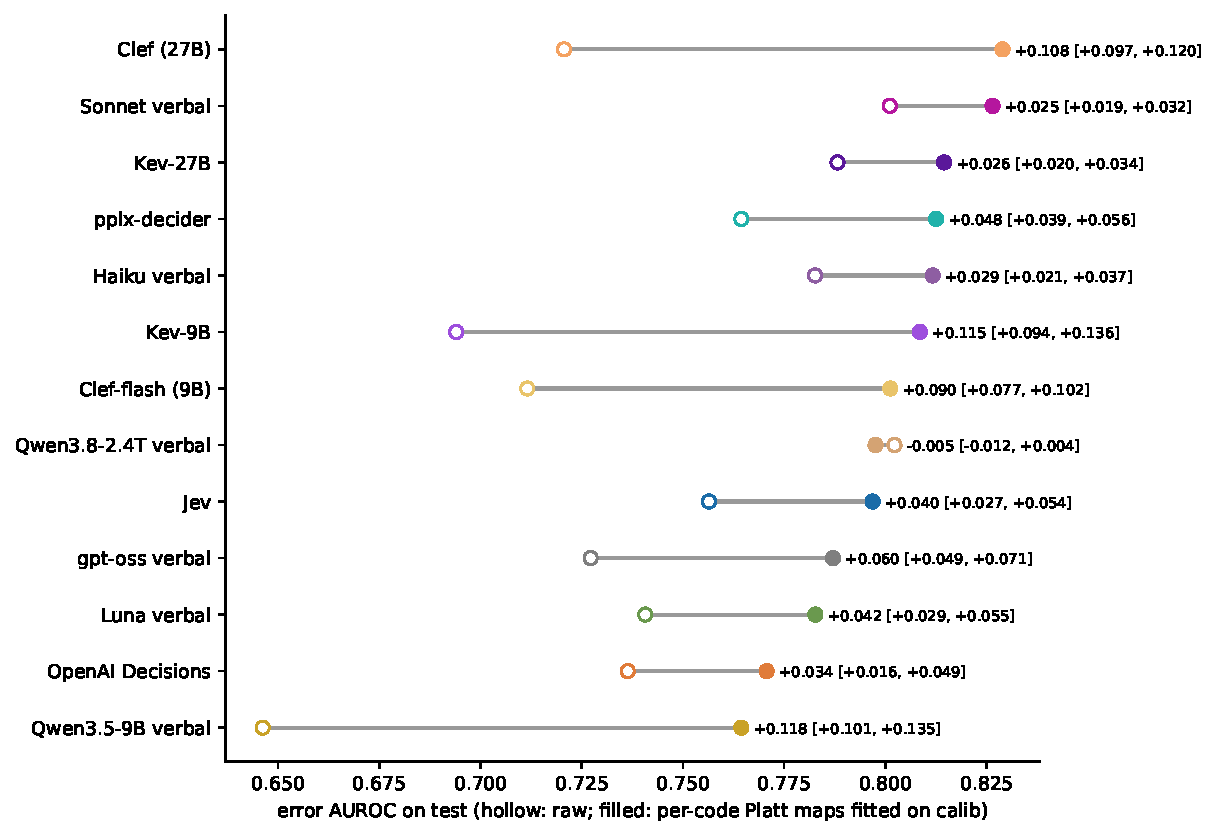
\includegraphics[width=0.8\linewidth]{fig10_per_code_recalibration.pdf}
  \caption{EQ3: error AUROC with raw confidence (hollow) and with per-code Platt maps fitted on the calibration split
  (filled), pooled over tasks, with cluster-bootstrap 95\% CIs for the gain, conditional on the fitted maps. Qwen3.8-2.4T ran
  on a subset whose calibration split is too small for per-code maps.}
  \label{fig:percode}
\end{figure}
\begin{table}[t]
\centering
\small
\caption{A3 (exploratory): per-code recalibration of confidence (error AUROC on test, pooled)}
\label{tab:tab10_per_code_recalibration}
\begin{adjustbox}{max width=\linewidth}
\begin{tabular}{lrrrrr}
\toprule
comparison & AUROC a & AUROC b & a -- b & 95\% CI low & 95\% CI high \\
\midrule
Jev: per-code calibrated - raw & 0.797 & 0.756 & 0.040 & 0.027 & 0.054 \\
OpenAI Decisions: per-code calibrated - raw & 0.771 & 0.736 & 0.034 & 0.016 & 0.049 \\
Clef (27B): per-code calibrated - raw & 0.829 & 0.721 & 0.108 & 0.097 & 0.120 \\
Clef-flash (9B): per-code calibrated - raw & 0.801 & 0.712 & 0.090 & 0.077 & 0.102 \\
pplx-decider: per-code calibrated - raw & 0.813 & 0.764 & 0.048 & 0.039 & 0.056 \\
Kev-9B: per-code calibrated - raw & 0.809 & 0.694 & 0.115 & 0.094 & 0.136 \\
Kev-27B: per-code calibrated - raw & 0.814 & 0.788 & 0.026 & 0.020 & 0.034 \\
Luna verbal: per-code calibrated - raw & 0.783 & 0.741 & 0.042 & 0.029 & 0.055 \\
Haiku verbal: per-code calibrated - raw & 0.812 & 0.783 & 0.029 & 0.021 & 0.037 \\
gpt-oss verbal: per-code calibrated - raw & 0.787 & 0.727 & 0.060 & 0.049 & 0.071 \\
Qwen3.5-9B verbal: per-code calibrated - raw & 0.764 & 0.646 & 0.118 & 0.101 & 0.135 \\
Sonnet verbal: per-code calibrated - raw & 0.826 & 0.801 & 0.025 & 0.019 & 0.032 \\
Qwen3.8-2.4T verbal: per-code calibrated - raw & 0.798 & 0.802 & -0.005 & -0.012 & 0.004 \\
Jev per-code (full calib) - Sonnet verbal raw & 0.797 & 0.801 & -0.004 & -0.018 & 0.008 \\
Jev raw - Sonnet verbal raw & 0.756 & 0.801 & -0.045 & -0.060 & -0.032 \\
Jev per-code - Sonnet verbal per-code (own calib) & 0.797 & 0.826 & -0.030 & -0.041 & -0.019 \\
Jev per-code (full calib) - Qwen3.8-2.4T verbal raw & 0.790 & 0.802 & -0.013 & -0.048 & 0.019 \\
Jev raw - Qwen3.8-2.4T verbal raw & 0.769 & 0.802 & -0.033 & -0.069 & -0.001 \\
Jev per-code - Qwen3.8-2.4T verbal per-code (own calib) & 0.790 & 0.798 & -0.008 & -0.043 & 0.024 \\
\bottomrule
\end{tabular}
\end{adjustbox}
\par\smallskip\footnotesize\raggedright Per-code Platt maps fitted on calib (codes with $\geq$ 50 calib decisions; others use the task map). CIs resample test clusters with the fitted maps held fixed, so they are conditional on those maps.
\end{table}

\begin{table}[t]
\centering
\small
\caption{Error AUROC from raw confidence, from the predicted code alone, and from per-code maps (pooled)}
\label{tab:tab22_category_only}
\begin{adjustbox}{max width=\linewidth}
\begin{tabular}{lrrr}
\toprule
signal & \makecell[br]{raw \\{} confidence} & \makecell[br]{predicted \\{} code only} & per-code maps \\
\midrule
Clef (27B) & 0.721 & 0.707 & 0.829 \\
Clef-flash (9B) & 0.712 & 0.693 & 0.801 \\
Haiku verbal & 0.783 & 0.696 & 0.812 \\
Jev & 0.756 & 0.714 & 0.797 \\
Kev-27B & 0.788 & 0.657 & 0.814 \\
Kev-9B & 0.694 & 0.713 & 0.809 \\
Luna verbal & 0.741 & 0.694 & 0.783 \\
OpenAI Decisions & 0.736 & 0.659 & 0.771 \\
gpt-oss verbal & 0.727 & 0.692 & 0.787 \\
pplx-decider & 0.764 & 0.691 & 0.813 \\
Sonnet verbal & 0.801 & 0.696 & 0.826 \\
\bottomrule
\end{tabular}
\end{adjustbox}
\par\smallskip\footnotesize\raggedright 'Predicted code only' scores each decision by the calibration accuracy of its predicted code (multi-label: of its code), with no confidence.
\end{table}

\FloatBarrier

\subsection{EQ5: configurations and cost}
We compared single coders, two-stage cascades, agreement gates and a seven-model committee, each at the API cost of its own
policy (\S\ref{sec:eq5}). The first table pools the naive and oracle rules over the five tasks; the second gives what corpus
LTT certifies on MFRC, with the share of comments a person still reads; the third tests selected differences between
configurations.

\begin{table}[t]
\centering
\small
\caption{A3 (exploratory): configurations under the naive and oracle rules, pooled over the five tasks}
\label{tab:tab08_cascades}
\begin{adjustbox}{max width=\linewidth}
\begin{tabular}{lrrlrl}
\toprule
configuration & \makecell[br]{naive: \\{} accepted} & naive: error & naive: USD/1k & \makecell[br]{oracle: \\{} accepted} & \makecell[bl]{oracle: \\{} USD/1k} \\
\midrule
Jev $\rightarrow$ human & 32.9 & 6.8 & 0.021 & 16.3 & 0.008 \\
OpenAI Decisions $\rightarrow$ human & 22.7 & 4.7 & 0.046 & 17.8 & 0.065 \\
Clef (27B) $\rightarrow$ human & 24.0 & 5.8 & 0.213 & 20.3 & 0.213 \\
Clef-flash (9B) $\rightarrow$ human & 25.4 & 7.0 & 0.080 & 20.7 & 0.080 \\
pplx-decider $\rightarrow$ human & 40.8 & 7.6 & 0.013 & 32.1 & 0.013 \\
Kev-9B $\rightarrow$ human & 23.9 & 6.3 & 0.073 & 19.2 & 0.058 \\
Kev-27B $\rightarrow$ human & 44.2 & 7.0 & 0.315 & 37.2 & 0.315 \\
Decision-model committee (7) $\rightarrow$ human & 37.5 & 7.2 & 0.849 & 30.9 & 0.849 \\
pplx-decider + Kev-27B agree $\rightarrow$ human & 42.7 & 6.8 & 0.334 & 40.5 & 0.334 \\
Jev + Kev-27B agree $\rightarrow$ human & 42.9 & 7.0 & 0.362 & 36.2 & 0.362 \\
Kev-27B $\rightarrow$ Sonnet verbal $\rightarrow$ human & 49.6 & 6.9 & 1.406 & 42.8 & 1.328 \\
Luna verbal $\rightarrow$ human & 20.2 & 4.6 & 0.082 & 16.2 & 0.066 \\
Haiku verbal $\rightarrow$ human & 16.1 & 3.2 & 1.137 & 16.8 & 1.906 \\
Sonnet verbal $\rightarrow$ human & 43.4 & 6.2 & 1.700 & 40.1 & 1.964 \\
Jev $\rightarrow$ Haiku verbal $\rightarrow$ human & 33.4 & 6.7 & 0.579 & 17.9 & 1.741 \\
Haiku verbal $\rightarrow$ Jev $\rightarrow$ human & 31.6 & 6.4 & 1.155 & 16.9 & 1.913 \\
Jev + Haiku verbal agree $\rightarrow$ human & 26.0 & 5.5 & 1.158 & 28.4 & 1.954 \\
Jev + Luna verbal agree $\rightarrow$ human & 34.3 & 6.6 & 0.130 & 17.8 & 0.131 \\
Jev $\rightarrow$ Sonnet verbal $\rightarrow$ human & 40.4 & 6.2 & 1.327 & 39.2 & 1.746 \\
Jev + Sonnet verbal agree $\rightarrow$ human & 43.1 & 6.5 & 1.736 & 39.1 & 2.011 \\
Haiku verbal + Sonnet verbal agree $\rightarrow$ human & 41.5 & 6.0 & 3.870 & 38.2 & 3.870 \\
\bottomrule
\end{tabular}
\end{adjustbox}
\par\smallskip\footnotesize\raggedright Accepted: percent of decisions auto-accepted; error: percent wrong among accepted decisions (tasks weighted equally); USD/1k: API cost per 1,000 segments under that policy. 'A + B agree' accepts where both give the same label (confidence = the lower).
\end{table}

\clearpage
\begin{table}[t]
\centering
\small
\caption{A3 (exploratory): configurations certified by corpus LTT on MFRC (percent; the only task where anything is certified when whole clusters are hand-coded)}
\label{tab:tab08b_cascades_certified}
\begin{adjustbox}{max width=\linewidth}
\begin{tabular}{lrrlrrr}
\toprule
configuration & \makecell[br]{certified: \\{} accepted} & error & \makecell[bl]{USD per 1k \\{} comments} & \makecell[br]{remainder \\{} comments \\{} still read} & \makecell[br]{all comments \\{} still read} & \makecell[br]{overall error \\{} vs \\{} adjudicated} \\
\midrule
Jev $\rightarrow$ human & 59.8 & 1.6 & 0.042 & 93.2 & 95.2 & 1.1 \\
OpenAI Decisions $\rightarrow$ human & 0.0 & -- & 0.000 & 100.0 & 100.0 & 0.2 \\
Clef (27B) $\rightarrow$ human & 82.3 & 3.1 & 0.245 & 73.3 & 81.4 & 2.6 \\
Clef-flash (9B) $\rightarrow$ human & 77.9 & 2.7 & 0.092 & 76.2 & 83.4 & 2.2 \\
pplx-decider $\rightarrow$ human & 77.1 & 2.3 & 0.029 & 73.2 & 81.3 & 1.9 \\
Kev-9B $\rightarrow$ human & 67.1 & 2.4 & 0.073 & 99.9 & 99.9 & 1.8 \\
Kev-27B $\rightarrow$ human & 76.6 & 2.1 & 0.315 & 84.6 & 89.3 & 1.7 \\
Decision-model committee (7) $\rightarrow$ human & 84.5 & 2.9 & 0.970 & 68.2 & 77.8 & 2.5 \\
pplx-decider + Kev-27B agree $\rightarrow$ human & 81.1 & 2.6 & 0.344 & 74.9 & 82.5 & 2.2 \\
Jev + Kev-27B agree $\rightarrow$ human & 75.7 & 2.2 & 0.357 & 78.1 & 84.7 & 1.8 \\
Kev-27B $\rightarrow$ Sonnet verbal $\rightarrow$ human & 82.3 & 2.5 & 4.141 & 74.0 & 81.9 & 2.1 \\
Luna verbal $\rightarrow$ human & 64.0 & 2.2 & 0.218 & 93.0 & 95.1 & 1.5 \\
Haiku verbal $\rightarrow$ human & 65.8 & 1.7 & 3.473 & 83.5 & 88.5 & 1.2 \\
Sonnet verbal $\rightarrow$ human & 82.7 & 2.5 & 4.521 & 65.7 & 76.1 & 2.2 \\
Jev $\rightarrow$ Haiku verbal $\rightarrow$ human & 66.5 & 1.7 & 3.513 & 83.1 & 88.2 & 1.3 \\
Haiku verbal $\rightarrow$ Jev $\rightarrow$ human & 66.5 & 1.8 & 3.509 & 83.1 & 88.2 & 1.3 \\
Jev + Haiku verbal agree $\rightarrow$ human & 63.3 & 1.8 & 3.516 & 90.2 & 93.2 & 1.3 \\
Jev + Luna verbal agree $\rightarrow$ human & 67.9 & 2.2 & 0.260 & 88.4 & 91.9 & 1.6 \\
Jev $\rightarrow$ Sonnet verbal $\rightarrow$ human & 77.0 & 1.9 & 4.479 & 78.4 & 85.0 & 1.5 \\
Jev + Sonnet verbal agree $\rightarrow$ human & 73.5 & 2.1 & 4.563 & 82.5 & 87.8 & 1.6 \\
Haiku verbal + Sonnet verbal agree $\rightarrow$ human & 74.2 & 2.3 & 7.995 & 75.3 & 82.8 & 1.8 \\
\bottomrule
\end{tabular}
\end{adjustbox}
\par\smallskip\footnotesize\raggedright Multi-stage configurations are certified jointly over the pipeline. Accepted, error and remainder comments still read refer to the uncoded remainder (the test split); a comment is still read if at least one of its decisions is left for a person. All comments still read adds the 608 hand-coded calibration comments to the numerator and denominator. Overall error vs adjudicated: certified decisions scored against the adjudicated reference, the rest taken as human-coded; human-only coding of MFRC has 0.2\% error against that reference.
\end{table}

\begin{table}[t]
\centering
\small
\caption{A3 (exploratory): paired configuration contrasts, accepted share a -- b in percentage points [95\% CI]}
\label{tab:tab09_cascade_contrasts}
\par\textit{A. Naive rule and oracle, pooled over the five tasks}\par\smallskip
\begin{adjustbox}{max width=\linewidth}
\begin{tabular}{llll}
\toprule
a & b & naive & oracle \\
\midrule
Jev $\rightarrow$ Luna verbal & Luna verbal & +13.0 [-0.7, +18.4] & +0.4 [-0.9, +10.8] \\
Jev $\rightarrow$ Haiku verbal & Haiku verbal & +17.3 [+0.9, +19.1] & +1.1 [-0.9, +9.6] \\
Jev $\rightarrow$ Haiku verbal & Jev & +0.5 [+0.0, +10.2] & +1.6 [+0.6, +17.2] \\
Jev $\rightarrow$ Haiku verbal & OpenAI Decisions $\rightarrow$ Haiku verbal & +9.2 [-5.3, +15.5] & -1.9 [-9.1, +5.7] \\
Jev & OpenAI Decisions & +10.3 [-5.0, +18.7] & -1.5 [-9.2, +4.9] \\
Jev + Haiku verbal agree & Jev $\rightarrow$ Haiku verbal & -7.4 [-11.3, +9.6] & +10.5 [-6.1, +10.3] \\
Jev + Haiku verbal agree & Jev & -6.9 [-10.0, +12.7] & +12.1 [-0.2, +14.7] \\
Jev + Haiku verbal agree & Haiku verbal & +10.0 [-1.6, +18.6] & +11.7 [-4.3, +12.0] \\
Jev + Luna verbal agree & Jev & +1.3 [-3.4, +13.4] & +1.5 [-2.0, +11.7] \\
Jev $\rightarrow$ Sonnet verbal & Sonnet verbal & -3.0 [-4.5, +2.3] & -0.9 [-2.7, +0.6] \\
Jev & Sonnet verbal & -10.5 [-28.3, -5.4] & -23.8 [-28.0, -12.1] \\
Jev + Haiku verbal agree & Sonnet verbal & -17.3 [-25.3, -5.7] & -11.7 [-19.7, -6.1] \\
Jev + Sonnet verbal agree & Sonnet verbal & -0.2 [-8.9, +3.1] & -1.0 [-4.6, +3.3] \\
Kev-27B & Jev & +11.3 [+6.3, +27.2] & +20.9 [+11.1, +27.6] \\
Decision-model committee (7) & Jev & +4.6 [+1.6, +21.1] & +14.6 [+5.2, +20.2] \\
Decision-model committee (7) & Sonnet verbal & -5.9 [-13.9, +1.6] & -9.2 [-12.8, -0.5] \\
pplx-decider + Kev-27B agree & Sonnet verbal & -0.7 [-9.5, +7.1] & +0.4 [-6.9, +8.7] \\
\bottomrule
\end{tabular}
\end{adjustbox}
\medskip
\par\textit{B. Corpus LTT on MFRC}\par\smallskip
\begin{adjustbox}{max width=\linewidth}
\begin{tabular}{lllr}
\toprule
a & b & corpus LTT & \makecell[br]{USD per 1k, a -- \\{} b} \\
\midrule
Jev $\rightarrow$ Luna verbal & Luna verbal & -4.8 [-64.6, +0.2] & 0.04 \\
Jev $\rightarrow$ Haiku verbal & Haiku verbal & +0.7 [-4.1, +8.1] & 0.04 \\
Jev $\rightarrow$ Haiku verbal & Jev & +6.7 [-3.1, +25.2] & 3.47 \\
Jev $\rightarrow$ Haiku verbal & OpenAI Decisions $\rightarrow$ Haiku verbal & +4.3 [-4.0, +62.7] & -0.13 \\
Jev & OpenAI Decisions & +59.8 [+42.9, +70.1] & 0.04 \\
Jev + Haiku verbal agree & Jev $\rightarrow$ Haiku verbal & -3.2 [-6.9, +1.7] & 0.00 \\
Jev + Haiku verbal agree & Jev & +3.5 [-6.6, +20.1] & 3.47 \\
Jev + Haiku verbal agree & Haiku verbal & -2.5 [-3.4, +3.4] & 0.04 \\
Jev + Luna verbal agree & Jev & +8.1 [-1.8, +23.3] & 0.22 \\
Jev $\rightarrow$ Sonnet verbal & Sonnet verbal & -5.7 [-9.3, +0.6] & -0.04 \\
Jev & Sonnet verbal & -22.9 [-42.3, -13.1] & -4.48 \\
Jev + Haiku verbal agree & Sonnet verbal & -19.4 [-23.5, -12.5] & -1.01 \\
Jev + Sonnet verbal agree & Sonnet verbal & -9.2 [-16.1, -7.5] & 0.04 \\
Kev-27B & Jev & +16.7 [+7.1, +38.2] & 0.27 \\
Decision-model committee (7) & Jev & +24.6 [+14.2, +40.9] & 0.93 \\
Decision-model committee (7) & Sonnet verbal & +1.8 [-8.3, +2.8] & -3.55 \\
pplx-decider + Kev-27B agree & Sonnet verbal & -1.6 [-10.0, +3.8] & -4.18 \\
\bottomrule
\end{tabular}
\end{adjustbox}
\par\smallskip\footnotesize\raggedright 1,000 clustered bootstrap replicates with thresholds refitted; related tasks share cluster draws. Naive and oracle: equal-weight means over the five tasks. Corpus LTT: MFRC only, the one task where it certifies anything when whole clusters are hand-coded. Every configuration ends with a person coding what it does not accept; 'A + B agree' accepts where both give the same label.
\end{table}

\FloatBarrier

\subsection{EQ6: validity checks}
Four checks bound specific threats to the results (\S\ref{sec:eq6}). Repeatability sends identical requests twice;
prompt sensitivity tries a second elicitation prompt for the LLM baselines; adjudication re-examines sampled disagreements
between coders and the human labels; and the memorization probe, with its decoy-name control, tests whether the LLMs
reproduce the public datasets. None of them proves validity; each addresses a particular alternative explanation. The model snapshot
records exactly what was called.

\begin{figure}[htbp]
  \centering
  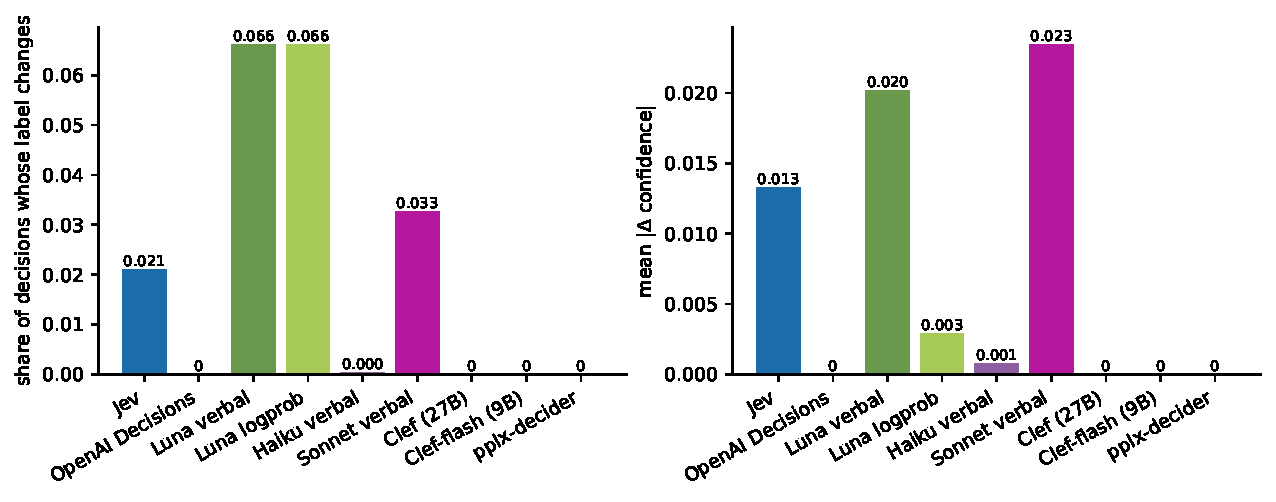
\includegraphics[width=\linewidth]{fig11_repeatability.pdf}
  \caption{EQ6: run-to-run repeatability. Identical requests were sent twice for 100 test segments per task. Left: share of
  decisions whose label changes. Right: mean absolute change in confidence. 0: no observed change in these repeats; $<$0.001:
  a nonzero value below display precision.}
  \label{fig:repeat}
\end{figure}
\begin{table}[t]
\centering
\small
\caption{Run-to-run repeatability (identical requests sent twice; 100 test segments per task; mean over tasks)}
\label{tab:tab11_repeatability}
\par\textit{A. How much the outputs change}\par\smallskip
\begin{adjustbox}{max width=\linewidth}
\begin{tabular}{lrrrrrr}
\toprule
signal & segments & decisions & \makecell[br]{label flip \\{} rate} & \makecell[br]{share \\{} identical} & mean |$\Delta$p| & \makecell[br]{mean |$\Delta$ \\{} confidence|} \\
\midrule
Jev & 100 & 240 & 0.021 & 0.612 & 0.008 & 0.013 \\
OpenAI Decisions & 100 & 240 & 0.000 & 1.000 & 0.000 & 0.000 \\
Luna verbal & 100 & 240 & 0.066 & 0.567 & 0.030 & 0.020 \\
Luna logprob & 100 & 240 & 0.066 & 0.455 & 0.031 & 0.003 \\
Haiku verbal & 100 & 240 & 0.000 & 0.989 & 0.001 & 0.001 \\
Sonnet verbal & 100 & 240 & 0.033 & 0.514 & 0.016 & 0.023 \\
Clef (27B) & 100 & 240 & 0.000 & 1.000 & 0.000 & 0.000 \\
Clef-flash (9B) & 100 & 240 & 0.000 & 1.000 & 0.000 & 0.000 \\
pplx-decider & 100 & 240 & 0.000 & 1.000 & 0.000 & 0.000 \\
\bottomrule
\end{tabular}
\end{adjustbox}
\medskip
\par\textit{B. Accuracy in each run, and where the changes fall}\par\smallskip
\begin{adjustbox}{max width=\linewidth}
\begin{tabular}{lrrr}
\toprule
signal & \makecell[br]{accuracy, \\{} run 1} & \makecell[br]{accuracy, \\{} run 2} & \makecell[br]{flips at low \\{} confidence \\{} (AUROC)} \\
\midrule
Jev & 0.743 & 0.741 & 0.967 \\
OpenAI Decisions & 0.723 & 0.723 & -- \\
Luna verbal & 0.742 & 0.742 & 0.874 \\
Luna logprob & 0.742 & 0.742 & 0.647 \\
Haiku verbal & 0.702 & 0.703 & 0.895 \\
Sonnet verbal & 0.764 & 0.765 & 0.921 \\
Clef (27B) & 0.693 & 0.693 & -- \\
Clef-flash (9B) & 0.685 & 0.685 & -- \\
pplx-decider & 0.759 & 0.759 & -- \\
\bottomrule
\end{tabular}
\end{adjustbox}
\par\smallskip\footnotesize\raggedright Flips at low confidence: AUROC of low confidence for the decisions whose label changed (-- : no changes).
\end{table}

\begin{table}[t]
\centering
\small
\caption{LLM prompt sensitivity: verbalized distribution vs canonical prompt (amendment v1.4)}
\label{tab:tab19_prompt_sensitivity}
\par\textit{A. Error ranking}\par\smallskip
\begin{adjustbox}{max width=\linewidth}
\begin{tabular}{llrrrrrr}
\toprule
task & signal & decisions & \makecell[br]{err. AUROC \\{} canonical} & \makecell[br]{err. AUROC \\{} distribution} & difference & lo & hi \\
\midrule
MFRC & Sonnet verbal & 1200 & 0.933 & 0.897 & -0.036 & -0.052 & -0.019 \\
MFRC & Haiku verbal & 1200 & 0.942 & 0.897 & -0.045 & -0.063 & -0.029 \\
AnnoMI client & Sonnet verbal & 150 & 0.750 & 0.726 & -0.024 & -0.074 & 0.018 \\
AnnoMI client & Haiku verbal & 150 & 0.733 & 0.776 & 0.043 & -0.041 & 0.136 \\
AnnoMI therapist & Sonnet verbal & 150 & 0.808 & 0.837 & 0.029 & -0.012 & 0.083 \\
AnnoMI therapist & Haiku verbal & 150 & 0.770 & 0.717 & -0.053 & -0.139 & 0.014 \\
TalkMoves teacher & Sonnet verbal & 150 & 0.817 & 0.747 & -0.070 & -0.135 & 0.000 \\
TalkMoves teacher & Haiku verbal & 150 & 0.747 & 0.767 & 0.021 & -0.080 & 0.120 \\
TalkMoves student & Sonnet verbal & 150 & 0.829 & 0.758 & -0.071 & -0.133 & -0.012 \\
TalkMoves student & Haiku verbal & 150 & 0.786 & 0.770 & -0.015 & -0.082 & 0.046 \\
Pooled & Sonnet verbal & 1800 & 0.827 & 0.793 & -0.034 & -0.056 & -0.011 \\
Pooled & Haiku verbal & 1800 & 0.796 & 0.786 & -0.010 & -0.045 & 0.022 \\
\bottomrule
\end{tabular}
\end{adjustbox}
\medskip
\par\textit{B. Agreement and calibration}\par\smallskip
\begin{adjustbox}{max width=\linewidth}
\begin{tabular}{llrrrrr}
\toprule
task & signal & decisions & $\kappa$ canonical & \makecell[br]{$\kappa$ \\{} distribution} & \makecell[br]{ECE \\{} canonical} & \makecell[br]{ECE \\{} distribution} \\
\midrule
MFRC & Sonnet verbal & 1200 & 0.346 & 0.365 & 0.048 & 0.031 \\
MFRC & Haiku verbal & 1200 & 0.166 & 0.174 & 0.128 & 0.076 \\
AnnoMI client & Sonnet verbal & 150 & 0.413 & 0.432 & 0.065 & 0.079 \\
AnnoMI client & Haiku verbal & 150 & 0.479 & 0.453 & 0.118 & 0.158 \\
AnnoMI therapist & Sonnet verbal & 150 & 0.751 & 0.715 & 0.053 & 0.083 \\
AnnoMI therapist & Haiku verbal & 150 & 0.634 & 0.661 & 0.155 & 0.158 \\
TalkMoves teacher & Sonnet verbal & 150 & 0.590 & 0.603 & 0.089 & 0.045 \\
TalkMoves teacher & Haiku verbal & 150 & 0.554 & 0.528 & 0.141 & 0.215 \\
TalkMoves student & Sonnet verbal & 150 & 0.539 & 0.548 & 0.118 & 0.090 \\
TalkMoves student & Haiku verbal & 150 & 0.445 & 0.430 & 0.261 & 0.330 \\
Pooled & Sonnet verbal & 1800 & 0.528 & 0.533 & 0.074 & 0.066 \\
Pooled & Haiku verbal & 1800 & 0.456 & 0.449 & 0.161 & 0.187 \\
\bottomrule
\end{tabular}
\end{adjustbox}
\par\smallskip\footnotesize\raggedright Same test items (first 150 per task). Difference = distribution -- canonical error AUROC, paired cluster bootstrap 95\% CI; related tasks share cluster draws.
\end{table}

\begin{table}[t]
\centering
\small
\caption{Who was right when a coder disagreed with the human label (adjudicated sample)}
\label{tab:tab12_adjudication}
\begin{adjustbox}{max width=\linewidth}
\begin{tabular}{llrrrrr}
\toprule
coder & verdicts & n & \makecell[br]{coder right, \\{} human wrong} & \makecell[br]{human right, \\{} coder wrong} & \makecell[br]{both \\{} defensible \\{} (codebook \\{} under-specified)} & neither right \\
\midrule
Jev & all & 117 & 0.598 & 0.325 & 0.068 & 0.009 \\
Jev & LLM panel & 90 & 0.622 & 0.289 & 0.089 & 0.000 \\
Jev & author & 27 & 0.519 & 0.444 & 0.000 & 0.037 \\
Luna verbal & all & 118 & 0.644 & 0.288 & 0.059 & 0.008 \\
Luna verbal & LLM panel & 84 & 0.667 & 0.250 & 0.083 & 0.000 \\
Luna verbal & author & 34 & 0.588 & 0.382 & 0.000 & 0.029 \\
Haiku verbal & all & 118 & 0.585 & 0.314 & 0.085 & 0.017 \\
Haiku verbal & LLM panel & 89 & 0.573 & 0.292 & 0.112 & 0.022 \\
Haiku verbal & author & 29 & 0.621 & 0.379 & 0.000 & 0.000 \\
gpt-oss verbal & all & 141 & 0.553 & 0.390 & 0.043 & 0.014 \\
gpt-oss verbal & LLM panel & 108 & 0.556 & 0.380 & 0.056 & 0.009 \\
gpt-oss verbal & author & 33 & 0.545 & 0.424 & 0.000 & 0.030 \\
\bottomrule
\end{tabular}
\end{adjustbox}
\par\smallskip\footnotesize\raggedright Shares of adjudicated disagreements on a high-confidence-enriched sample drawn from six label sources (Jev in both formats, Luna, Haiku, gpt-oss and Sonnet's subset run); the four coders shown have enough disagreements to break down. The panel resolved the items on which its two members agreed; the author resolved 36 items the panel disputed plus a 12-item audit of panel-agreed items (deviations 2--3).
\end{table}

\begin{figure}[htbp]
  \centering
  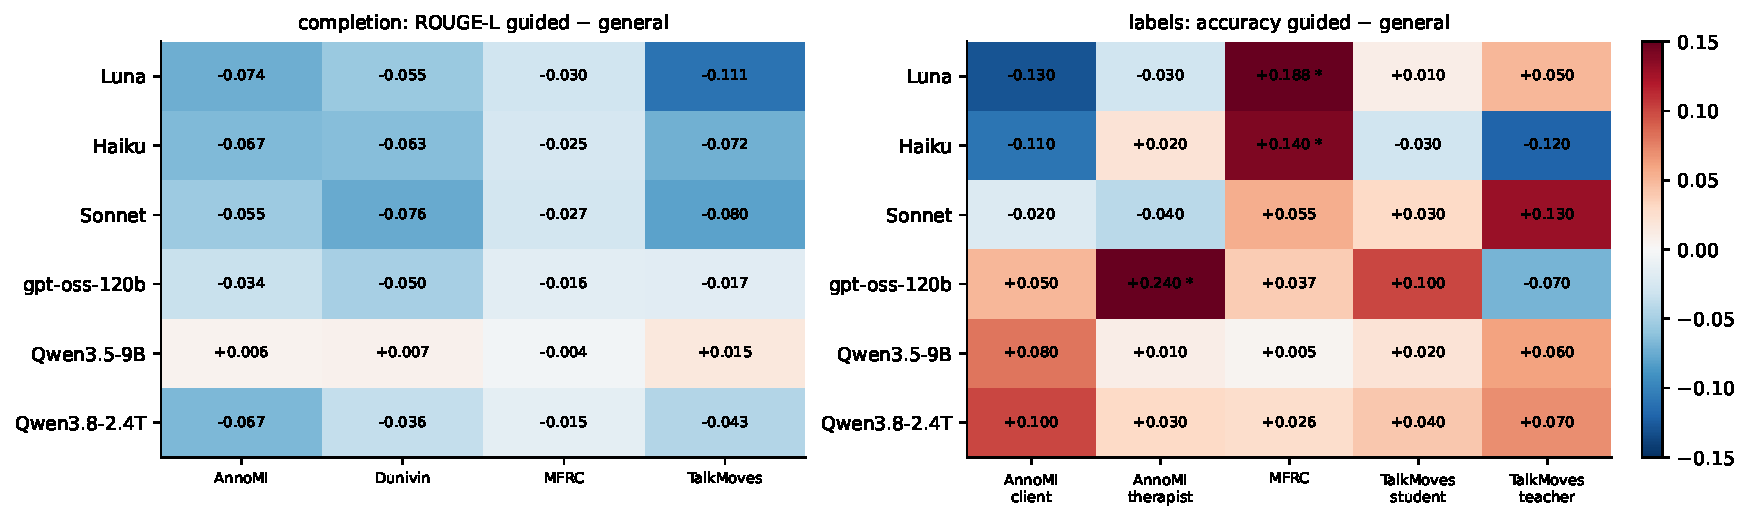
\includegraphics[width=\linewidth]{fig14_memorization.pdf}
  \caption{EQ6: memorization probe. Change in completion overlap (left, ROUGE-L) and label recall (right, accuracy) when
  the dataset is named, relative to an unnamed prompt. Asterisks mark cells flagged by the pre-specified rule;
  Table~\ref{tab:tab17_memorization_followups} gives the decoy control.}
  \label{fig:mem}
\end{figure}
\begin{table}[t]
\centering
\small
\caption{Memorization probe: completing the second half of dataset items, overlap with the true continuation (amendment v1.3)}
\label{tab:tab15_memorization_completion}
\begin{adjustbox}{max width=\linewidth}
\begin{tabular}{llrrrrr}
\toprule
model & dataset & items & \makecell[br]{ROUGE-L, \\{} named} & \makecell[br]{ROUGE-L, \\{} unnamed} & difference & \makecell[br]{p \\{} (Bonferroni)} \\
\midrule
Haiku & annomi & 100 & 0.079 & 0.146 & -0.067 & 1.000 \\
Haiku & dunivin & 100 & 0.080 & 0.144 & -0.063 & 1.000 \\
Haiku & mfrc & 100 & 0.080 & 0.105 & -0.025 & 1.000 \\
Haiku & talkmoves & 100 & 0.082 & 0.155 & -0.072 & 1.000 \\
Luna & annomi & 100 & 0.082 & 0.156 & -0.074 & 1.000 \\
Luna & dunivin & 100 & 0.095 & 0.151 & -0.055 & 1.000 \\
Luna & mfrc & 100 & 0.082 & 0.111 & -0.030 & 1.000 \\
Luna & talkmoves & 100 & 0.063 & 0.174 & -0.111 & 1.000 \\
gpt-oss-120b & annomi & 100 & 0.057 & 0.090 & -0.034 & 1.000 \\
gpt-oss-120b & dunivin & 100 & 0.016 & 0.066 & -0.050 & 1.000 \\
gpt-oss-120b & mfrc & 100 & 0.038 & 0.055 & -0.016 & 1.000 \\
gpt-oss-120b & talkmoves & 100 & 0.049 & 0.066 & -0.017 & 1.000 \\
Qwen3.5-9B & annomi & 100 & 0.142 & 0.137 & 0.006 & 1.000 \\
Qwen3.5-9B & dunivin & 100 & 0.143 & 0.137 & 0.007 & 1.000 \\
Qwen3.5-9B & mfrc & 100 & 0.098 & 0.102 & -0.004 & 1.000 \\
Qwen3.5-9B & talkmoves & 100 & 0.163 & 0.148 & 0.015 & 1.000 \\
Qwen3.8-2.4T & annomi & 100 & 0.083 & 0.150 & -0.067 & 1.000 \\
Qwen3.8-2.4T & dunivin & 100 & 0.112 & 0.148 & -0.036 & 1.000 \\
Qwen3.8-2.4T & mfrc & 100 & 0.086 & 0.101 & -0.015 & 1.000 \\
Qwen3.8-2.4T & talkmoves & 100 & 0.125 & 0.168 & -0.043 & 1.000 \\
Sonnet & annomi & 100 & 0.098 & 0.153 & -0.055 & 1.000 \\
Sonnet & dunivin & 100 & 0.099 & 0.175 & -0.076 & 1.000 \\
Sonnet & mfrc & 100 & 0.089 & 0.116 & -0.027 & 1.000 \\
Sonnet & talkmoves & 100 & 0.076 & 0.156 & -0.080 & 1.000 \\
\bottomrule
\end{tabular}
\end{adjustbox}
\par\smallskip\footnotesize\raggedright Named: the dataset is named and the exact original text requested. Unnamed: plain continuation. Difference: named -- unnamed mean ROUGE-L; p: one-sided Wilcoxon signed-rank test for named > unnamed, Bonferroni-adjusted. Near-verbatim matches are in Table~\ref{tab:tab15b_memorization_verbatim}.
\end{table}

\begin{table}[t]
\centering
\small
\caption{Memorization probe: near-verbatim reproduction (counts of items, amendment v1.3)}
\label{tab:tab15b_memorization_verbatim}
\begin{adjustbox}{max width=\linewidth}
\begin{tabular}{llrrrrr}
\toprule
model & dataset & items & \makecell[br]{near-verbatim \\{} items, named} & \makecell[br]{near-verbatim \\{} items, \\{} unnamed} & \makecell[br]{longest run, \\{} named \\{} (words)} & flagged \\
\midrule
Haiku & annomi & 100 & 0 & 0 & 3 & no \\
Haiku & dunivin & 100 & 0 & 0 & 2 & no \\
Haiku & mfrc & 100 & 0 & 0 & 3 & no \\
Haiku & talkmoves & 100 & 0 & 1 & 3 & no \\
Luna & annomi & 100 & 0 & 0 & 2 & no \\
Luna & dunivin & 100 & 1 & 0 & 45 & no \\
Luna & mfrc & 100 & 0 & 0 & 2 & no \\
Luna & talkmoves & 100 & 0 & 0 & 4 & no \\
gpt-oss-120b & annomi & 100 & 0 & 0 & 2 & no \\
gpt-oss-120b & dunivin & 100 & 0 & 0 & 1 & no \\
gpt-oss-120b & mfrc & 100 & 0 & 0 & 2 & no \\
gpt-oss-120b & talkmoves & 100 & 0 & 0 & 3 & no \\
Qwen3.5-9B & annomi & 100 & 0 & 0 & 6 & no \\
Qwen3.5-9B & dunivin & 100 & 0 & 0 & 8 & no \\
Qwen3.5-9B & mfrc & 100 & 0 & 0 & 4 & no \\
Qwen3.5-9B & talkmoves & 100 & 1 & 1 & 10 & no \\
Qwen3.8-2.4T & annomi & 100 & 0 & 0 & 4 & no \\
Qwen3.8-2.4T & dunivin & 100 & 0 & 1 & 8 & no \\
Qwen3.8-2.4T & mfrc & 100 & 0 & 0 & 4 & no \\
Qwen3.8-2.4T & talkmoves & 100 & 0 & 0 & 5 & no \\
Sonnet & annomi & 100 & 0 & 0 & 3 & no \\
Sonnet & dunivin & 100 & 0 & 1 & 9 & no \\
Sonnet & mfrc & 100 & 0 & 0 & 3 & no \\
Sonnet & talkmoves & 100 & 0 & 0 & 2 & no \\
\bottomrule
\end{tabular}
\end{adjustbox}
\par\smallskip\footnotesize\raggedright Near-verbatim: a run of $\geq$ 10 identical words covering $\geq$ 50\% of the true continuation; counts of the 100 items. Longest run: the longest identical run under the named prompt only. Flagged: the pre-specified rule (Bonferroni p < 0.05 for named > unnamed in Table~\ref{tab:tab15_memorization_completion}, or $\geq$ 2 near-verbatim items under the named prompt). Matches include a predictable counting sequence (TalkMoves) and Du Bois quotations (Dunivin).
\end{table}

\begin{table}[t]
\centering
\small
\caption{Memorization probe: recalling annotated labels without the codebook (amendment v1.3)}
\label{tab:tab16_memorization_labels}
\begin{adjustbox}{max width=\linewidth}
\begin{tabular}{llrrrrrr}
\toprule
model & task & items & \makecell[br]{accuracy \\{} guided} & \makecell[br]{accuracy \\{} general} & difference & \makecell[br]{p \\{} (Bonferroni)} & \makecell[br]{evidence of \\{} label leakage} \\
\midrule
Haiku & AnnoMI client & 100 & 0.510 & 0.620 & -0.110 & 1.000 & no \\
Haiku & AnnoMI therapist & 100 & 0.580 & 0.560 & 0.020 & 1.000 & no \\
Haiku & MFRC & 100 & 0.314 & 0.174 & 0.140 & 0.014 & yes \\
Haiku & TalkMoves student & 100 & 0.440 & 0.470 & -0.030 & 1.000 & no \\
Haiku & TalkMoves teacher & 100 & 0.160 & 0.280 & -0.120 & 1.000 & no \\
Luna & AnnoMI client & 100 & 0.580 & 0.710 & -0.130 & 1.000 & no \\
Luna & AnnoMI therapist & 100 & 0.530 & 0.560 & -0.030 & 1.000 & no \\
Luna & MFRC & 100 & 0.408 & 0.220 & 0.188 & 0.015 & yes \\
Luna & TalkMoves student & 100 & 0.530 & 0.520 & 0.010 & 1.000 & no \\
Luna & TalkMoves teacher & 100 & 0.520 & 0.470 & 0.050 & 1.000 & no \\
gpt-oss-120b & AnnoMI client & 100 & 0.560 & 0.510 & 0.050 & 1.000 & no \\
gpt-oss-120b & AnnoMI therapist & 100 & 0.680 & 0.440 & 0.240 & 0.004 & yes \\
gpt-oss-120b & MFRC & 100 & 0.260 & 0.223 & 0.037 & 1.000 & no \\
gpt-oss-120b & TalkMoves student & 100 & 0.510 & 0.410 & 0.100 & 0.621 & no \\
gpt-oss-120b & TalkMoves teacher & 100 & 0.200 & 0.270 & -0.070 & 1.000 & no \\
Qwen3.5-9B & AnnoMI client & 100 & 0.720 & 0.640 & 0.080 & 1.000 & no \\
Qwen3.5-9B & AnnoMI therapist & 100 & 0.570 & 0.560 & 0.010 & 1.000 & no \\
Qwen3.5-9B & MFRC & 100 & 0.174 & 0.170 & 0.005 & 1.000 & no \\
Qwen3.5-9B & TalkMoves student & 100 & 0.420 & 0.400 & 0.020 & 1.000 & no \\
Qwen3.5-9B & TalkMoves teacher & 100 & 0.360 & 0.300 & 0.060 & 1.000 & no \\
Qwen3.8-2.4T & AnnoMI client & 100 & 0.720 & 0.620 & 0.100 & 0.959 & no \\
Qwen3.8-2.4T & AnnoMI therapist & 100 & 0.730 & 0.700 & 0.030 & 1.000 & no \\
Qwen3.8-2.4T & MFRC & 100 & 0.185 & 0.160 & 0.026 & 1.000 & no \\
Qwen3.8-2.4T & TalkMoves student & 100 & 0.490 & 0.450 & 0.040 & 1.000 & no \\
Qwen3.8-2.4T & TalkMoves teacher & 100 & 0.280 & 0.210 & 0.070 & 1.000 & no \\
Sonnet & AnnoMI client & 100 & 0.720 & 0.740 & -0.020 & 1.000 & no \\
Sonnet & AnnoMI therapist & 100 & 0.730 & 0.770 & -0.040 & 1.000 & no \\
Sonnet & MFRC & 100 & 0.573 & 0.518 & 0.055 & 1.000 & no \\
Sonnet & TalkMoves student & 100 & 0.590 & 0.560 & 0.030 & 1.000 & no \\
Sonnet & TalkMoves teacher & 100 & 0.630 & 0.500 & 0.130 & 0.287 & no \\
\bottomrule
\end{tabular}
\end{adjustbox}
\par\smallskip\footnotesize\raggedright Accuracy against the majority label (Jaccard for MFRC). Guided names the dataset and asks what its annotators assigned.
\end{table}

\begin{table}[t]
\centering
\small
\caption{Flagged label-probe cells: decoy-name control and coding accuracy on 'recalled' items}
\label{tab:tab17_memorization_followups}
\par\textit{A. Label recall with the real name, a decoy name and no name}\par\smallskip
\begin{adjustbox}{max width=\linewidth}
\begin{tabular}{llrrrrrrr}
\toprule
model & task & items & real name & decoy name & no name & real -- decoy & \makecell[br]{p (real > \\{} decoy)} & \makecell[br]{p \\{} (Bonferroni, \\{} 3 cells)} \\
\midrule
Haiku & MFRC & 100 & 0.314 & 0.246 & 0.174 & 0.068 & 0.021 & 0.063 \\
Luna & MFRC & 100 & 0.408 & 0.280 & 0.220 & 0.128 & 0.012 & 0.035 \\
gpt-oss-120b & AnnoMI therapist & 100 & 0.680 & 0.650 & 0.440 & 0.030 & 0.304 & 0.911 \\
\bottomrule
\end{tabular}
\end{adjustbox}
\medskip
\par\textit{B. Coding accuracy on 'recalled' and other items}\par\smallskip
\begin{adjustbox}{max width=\linewidth}
\begin{tabular}{llrrrrr}
\toprule
model & task & \makecell[br]{recalled \\{} items} & other items & \makecell[br]{coding \\{} accuracy, \\{} recalled} & \makecell[br]{coding \\{} accuracy, \\{} other} & \makecell[br]{p (recalled \\{} > other)} \\
\midrule
Haiku & MFRC & 22 & 78 & 0.841 & 0.782 & 0.085 \\
Luna & MFRC & 35 & 65 & 0.868 & 0.883 & 0.779 \\
gpt-oss-120b & AnnoMI therapist & 33 & 67 & 0.970 & 0.672 & 0.000 \\
\bottomrule
\end{tabular}
\end{adjustbox}
\par\smallskip\footnotesize\raggedright Decoy: the same dataset description with a fictitious name (deviation 14). Memory is supported only if the real name beats the decoy. Recalled items: guided better than no name. Coding accuracy is the model's RQ1 accuracy on those items.
\end{table}

\begin{table}[t]
\centering
\small
\caption{Model snapshot: what was called, which version answered, and when}
\label{tab:tab18_model_snapshot}
\begin{adjustbox}{max width=\linewidth}
\begin{tabular}{llllrll}
\toprule
coder & provider & \makecell[bl]{model \\{} requested} & \makecell[bl]{version \\{} returned} & \makecell[br]{calls (all \\{} arms)} & \makecell[bl]{first call \\{} (UTC)} & \makecell[bl]{last call \\{} (UTC)} \\
\midrule
Jev & typesafe & jev-1.13.0 & jev-1.13.0 & 65995 & 2026-10-10 & 2026-10-11 \\
OpenAI Decisions & openai decisions & gpt-6-luna & gpt-6-luna & 65993 & 2026-10-11 & 2026-10-11 \\
Clef & cloudflare & @cf/cloudflare/clef & clef & 14617 & 2026-10-11 & 2026-10-11 \\
Clef-flash & cloudflare & @cf/cloudflare/clef-flash & clef-flash & 65993 & 2026-10-11 & 2026-10-11 \\
pplx-decider & perplexity & pplx-decider-v1.1-27b & pplx-decider-v1.1-27b & 65993 & 2026-10-11 & 2026-10-11 \\
Kev-9B & kev & jaredpalmer/kev-9b & kev-latest & 51368 & 2026-10-11 & 2026-10-11 \\
Kev-27B & kev & jaredpalmer/kev-27b & kev-latest & 14117 & 2026-10-11 & 2026-10-11 \\
Luna & openai & gpt-6-luna & gpt-6-luna & 13905 & 2026-10-10 & 2026-10-11 \\
Haiku & anthropic & claude-haiku-4-5 & claude-haiku-4-5-20251001 & 11280 & 2026-10-10 & 2026-10-12 \\
Sonnet & anthropic & claude-sonnet-5-5 & claude-sonnet-5-5 & 12437 & 2026-10-10 & 2026-10-12 \\
gpt-oss-120b & together & openai/gpt-oss-120b & openai/gpt-oss-120b & 10030 & 2026-10-10 & 2026-10-11 \\
Qwen3.5-9B & together & Qwen/Qwen3.5-9B & Qwen/Qwen3.5-9B & 9930 & 2026-10-11 & 2026-10-11 \\
Qwen3.8-2.4T & together & Qwen/Qwen3.8-2.4T-A95B & Qwen/Qwen3.8-2.4T-A95B & 3281 & 2026-10-11 & 2026-10-11 \\
\bottomrule
\end{tabular}
\end{adjustbox}
\par\smallskip\footnotesize\raggedright Several APIs were in public beta (OpenAI Decisions from 2026-10-06; decision models launched September--October 2026). Kev weights: Hugging Face revisions db029f0 (kev-9b) and af0e6d5 (kev-27b), the latest on the call dates; kev package commit fc4a17e. Results describe these versions on these dates; the released harness allows re-running against later versions.
\end{table}

\FloatBarrier

\clearpage
\section{Requests}
\label{app:prompts}

\paragraph{LLM prompt} (canonical; AnnoMI client format; the exchange shown is invented for illustration, since AnnoMI's
text is not redistributed). The system prompt carries the codebook; option letters and
their order are shared with the decision-model request.
{\footnotesize\verbatiminput{sections/prompt_llm.txt}}

\paragraph{Decision-model request} (the same item). Jev, Clef, pplx-decider and Kev receive this exact JSON. OpenAI
Decisions receives the same content mapped to its choice and predicate types.
{\footnotesize\verbatiminput{sections/prompt_jev.txt}}

\section{Memorization probe}
\label{app:memorization}

For each of MFRC, AnnoMI, TalkMoves and Dunivin we drew 100 items of at least 30 words (20 for TalkMoves), with a fixed
seed. The model saw the first half of the words (plus the previous turn for dialogue). The \emph{guided} prompt named the
dataset and its citation and asked for the exact original continuation. The \emph{general} prompt asked only for a
continuation \citep{golchin2024time}. We scored word-level ROUGE-L \citep{lin2004rouge} and the longest common run of words,
and called a completion near-verbatim if the run was at least 10 words and covered at least half of the true continuation.
The label probe gave the item and the bare code labels, without definitions. The decoy control replaced the dataset name and
citation with a fictitious one while keeping the description. Tables~\ref{tab:tab15_memorization_completion}--\ref{tab:tab17_memorization_followups}
report all cells.
